\PassOptionsToPackage{english}{babel}
\documentclass[esp]{FCEFyN-class}
\usepackage{bm,placeins}
\setkeys{Gin}{draft=false}
\captionsetup[figure]{skip=8pt}
\setlength{\belowcaptionskip}{4pt}
\setlength{\floatsep}{18pt plus 4pt minus 2pt}
\setlength{\textfloatsep}{18pt plus 4pt minus 2pt}
\setlength{\dblfloatsep}{18pt plus 4pt minus 2pt}
\setlength{\dbltextfloatsep}{18pt plus 4pt minus 2pt}
\makeatletter
\setlength{\@dblfpsep}{24pt plus 2fil}
\makeatother
\newcommand{\I}{\bm I}
\newcommand{\Sx}[1]{[\bm{#1}]_\times}
\newcommand{\dd}{\mathrm d}
\newcommand{\tr}{\mathsf T}
\title{Formulación matemática de la dinámica estructural de un aerogenerador con rotación prescrita\\Mathematical formulation of wind turbine structural dynamics with prescribed rotation}
\shorttitle{Dinámica estructural de un aerogenerador}
\author[1,2,3]{Diego F. Turello}
\author[1]{Mauro S. Maza}
\author[4]{Nicolás Andrés Useche Castillo}
\author[4]{\authorcr Omar Lopez}
\author[1,2]{Sergio Preidikman}
\author[1,2]{Federico Pinto}
\affil[1]{Departamento de Estructuras, Facultad de Ciencias Exactas, Físicas y Naturales, Universidad Nacional de Córdoba, Córdoba, Argentina}
\affil[2]{Instituto de Estudios Avanzados en Ingeniería y Tecnología, UNC--CONICET, Córdoba, Argentina}
\affil[3]{Universidad Tecnológica Nacional, Facultad Regional Santa Fe, Santa Fe, Argentina}
\affil[4]{Departamento de Ingeniería Mecánica, Universidad de los Andes, Bogotá, Colombia}
\firstauthor{Turello}
\contactauthor{Diego F. Turello}
\email{diego.turello@unc.edu.ar}
\mailingaddress{Departamento de Estructuras, FCEFyN--UNC, Córdoba, Argentina}
\phonenumber{no consignado}
% Datos reservados al proceso editorial; no se asignan fechas ni volumen.
\thisvolume{--}\thisnumber{--}\thismonth{}\thisyear{}
\receptiondate{--}\acceptancedate{--}\publicationdate{--}
\hypersetup{pdftitle={Formulación matemática de la dinámica estructural de un aerogenerador con rotación prescrita},pdfauthor={Diego F. Turello; Mauro S. Maza; Nicolás Andrés Useche Castillo; Omar Lopez; Sergio Preidikman; Federico Pinto}}
\begin{document}
\selectlanguage{spanish}
\resumen{Se desarrolla un modelo matemático de la dinámica estructural de un aerogenerador de eje horizontal cuyo rotor tiene velocidad angular nominal prescrita. La torre y las tres palas se representan mediante vigas de Timoshenko, mientras que la góndola y el cubo se idealizan como cuerpos rígidos conectados elásticamente. La formulación distingue la configuración material de referencia, el movimiento nominal y las perturbaciones estructurales, y define los sistemas de referencia de cada componente. A partir de esta cinemática se obtienen las propiedades de masa y rigidez, las relaciones de compatibilidad y las ecuaciones discretas. La energía cinética permite deducir de manera consistente los efectos giroscópicos y las contribuciones del giro al equilibrio y a su linealización, considerando excentricidad y anisotropía de la distribución de masa. Se conservan las derivadas temporales de los cambios de coordenadas y de los vínculos entre el cubo y las raíces de las palas. Finalmente, se incorporan las acciones gravitatorias, aerodinámicas y sísmicas, y se establecen los problemas de vibración y respuesta transitoria alrededor de un estado de operación. El modelo diferencia el equilibrio relativo del análisis local a azimut fijo y explicita las hipótesis necesarias para cada descripción.}
\palabrasclave{Aerogeneradores, Dinámica estructural, Cinemática, Efectos giroscópicos, Elementos finitos.}
\abstract{\foreignlanguage{english}{A mathematical model is developed for the structural dynamics of a horizontal-axis wind turbine with prescribed nominal rotor angular velocity. The tower and three blades are represented by Timoshenko beams, whereas the nacelle and hub are idealized as elastically connected rigid bodies. The formulation distinguishes the material reference configuration, nominal motion, and structural perturbations, and defines the reference frames attached to each component. Mass and stiffness properties, compatibility relations, and discrete equations follow from this kinematic description. Kinetic energy provides a consistent derivation of gyroscopic effects and the contributions of prescribed rotation to equilibrium and its linearization, accounting for mass eccentricity and anisotropy. Time derivatives of coordinate transformations and hub--blade-root constraints are retained. Gravitational, aerodynamic, and seismic actions are then introduced, and vibration and transient-response problems are formulated about an operating state. The model distinguishes relative equilibrium from a local frozen-azimuth analysis and states the assumptions required by each description.}}
\keywords{Wind turbines, Structural dynamics, Kinematics, Gyroscopic effects, Finite elements.}
\maketitle
\thispagestyle{fancy}
\blfootnote{\fontsize{8}{11}\selectfont Autor de correspondencia: Diego F. Turello, \href{mailto:diego.turello@unc.edu.ar}{diego.turello@unc.edu.ar}.}
\clearpage
\section{Introducción}
La respuesta estructural de un aerogenerador de eje horizontal depende de la flexibilidad de la torre y las palas, del movimiento del rotor y de las acciones transmitidas por el viento y la cimentación. Su descripción requiere combinar componentes que giran con otros que permanecen nominalmente estacionarios. Esta coexistencia hace necesario especificar tanto la configuración respecto de la cual se mide la deformación como el sistema de referencia en el que se expresan posiciones, velocidades y fuerzas.

Los trabajos de \citet{maza2014} y \citet{turello2023} proporcionan antecedentes del análisis aeroelástico y de la interacción suelo--estructura en aerogeneradores. La mecánica del continuo establece la distinción entre movimiento y deformación \citep{holzapfel2000}, mientras que la dinámica de sistemas multicuerpo organiza las relaciones entre componentes rígidos y flexibles \citep{shabana2013}. Las formulaciones de vigas con rotaciones finitas \citep{simo1985} constituyen una referencia cinemática; el modelo aquí considerado se especializa a pequeñas deformaciones y pequeñas rotaciones estructurales respecto de una rotación nominal que puede ser arbitrariamente grande.

El objetivo es establecer una formulación estructural en la que la cinemática, las propiedades físicas y las ecuaciones de movimiento compartan una misma convención. La exposición comienza por los cuerpos y sus sistemas de referencia, continúa con las propiedades seccionales y la discretización y deduce después las contribuciones del giro prescrito. Para ello se distingue la descomposición de la energía cinética según el grado en las velocidades generalizadas de su posterior expansión alrededor del estado de operación \citep{meirovitch1997}. El desarrollo se completa con los vínculos cinemáticos, las cargas externas y los problemas de vibración y respuesta transitoria.

\section{Descripción del sistema y cinemática}
\label{sec:cinematica}
Se considera un aerogenerador de tres palas, orientado en la dirección del viento medio, con eje nominal horizontal. La torre y las palas son deformables; la góndola y el conjunto cubo--nariz se consideran rígidos. La conexión entre góndola y cubo permite pequeños desplazamientos y giros relativos mediante rigideces y amortiguamientos equivalentes. Las uniones entre el cubo y las raíces de las palas son rígidas. La figura~\ref{fig:modelo} identifica los componentes; el movimiento de base se transmite a través de la torre.

\begin{figure}[tp]
\centering
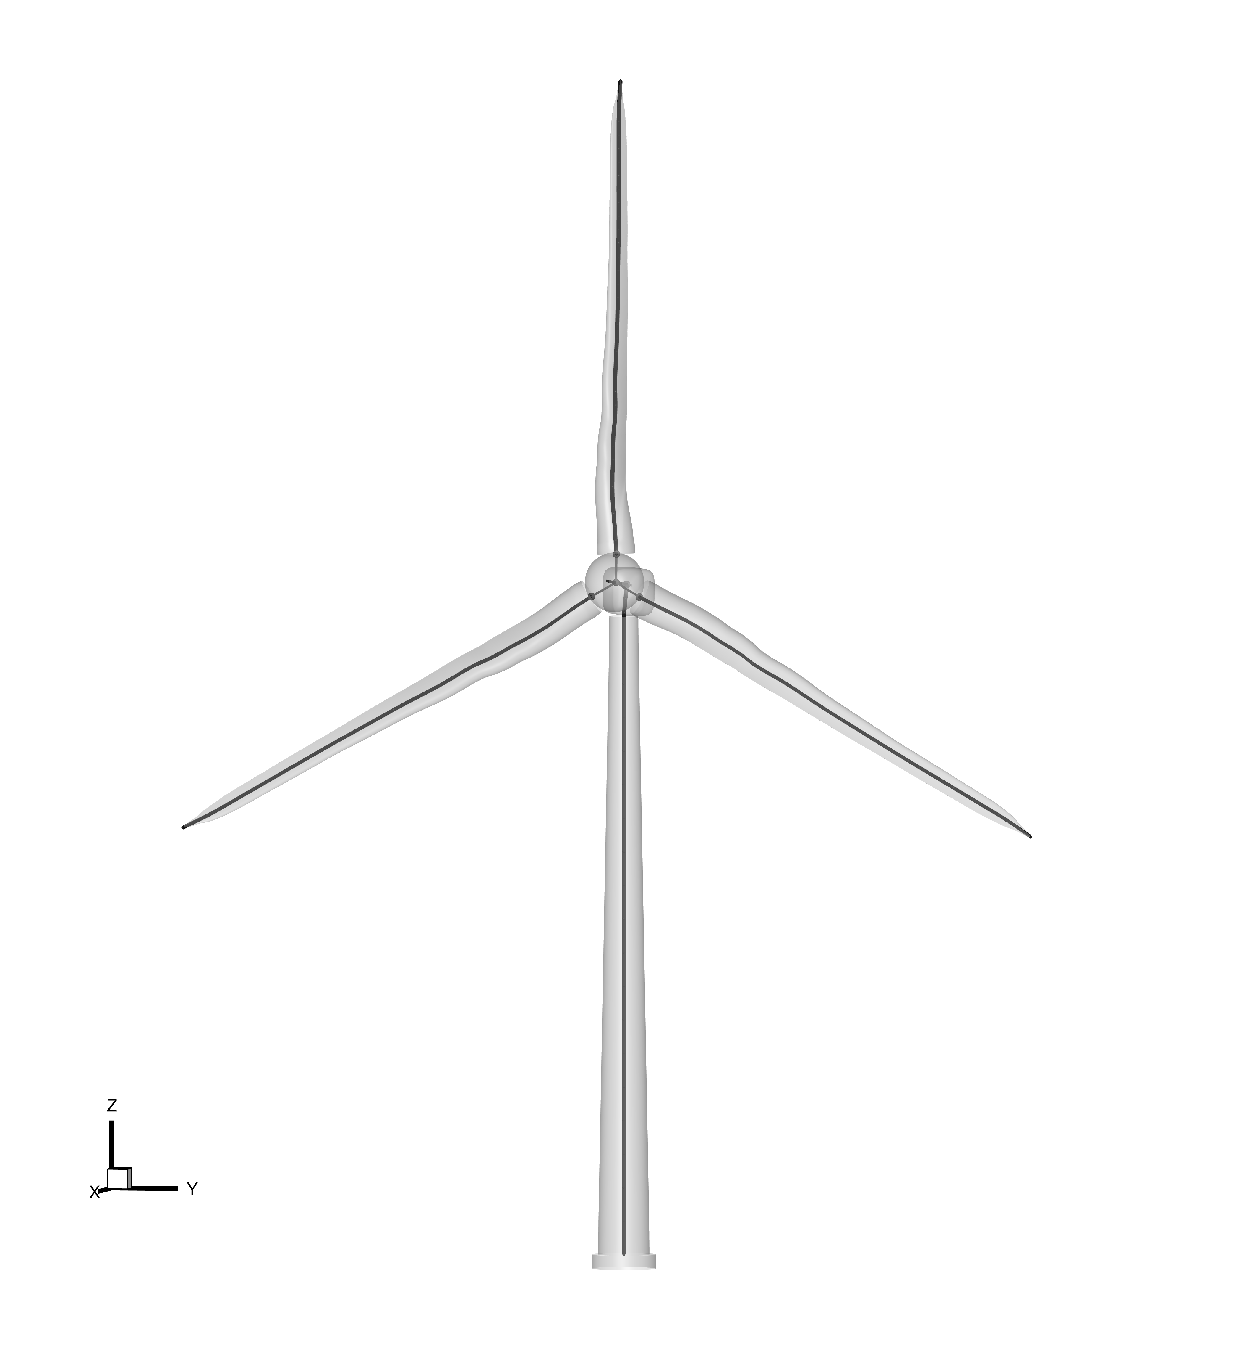
\includegraphics[trim={36.855bp 32.226bp 94.327bp 32.084bp},clip,width=.92\columnwidth,height=.31\textheight,keepaspectratio]{figures/tecplot/turbina_3d.pdf}
\caption{Idealización estructural del aerogenerador: torre y palas flexibles, góndola y cubo rígidos. Las líneas y los nodos interiores identifican el modelo de vigas. Las envolventes exteriores son ilustrativas y no constituyen una malla de sólidos ni geometría CAD.}\label{fig:modelo}
\end{figure}

\subsection{Configuraciones y convención de componentes}
Un cuerpo material es el conjunto de partículas que constituye un componente. Su configuración de referencia $\mathcal B_0$ asigna a cada partícula una posición $\bm X$; su configuración actual $\mathcal B_t$ contiene las posiciones ocupadas en el instante $t$. El movimiento se expresa mediante

\begin{equation}
\bm x=\bm\chi(\bm X,t),\qquad
\bm U(\bm X,t)=\bm\chi(\bm X,t)-\bm X.
\label{eq:configuraciones}
\end{equation}

La referencia se toma como la geometría de montaje sin deformación elástica de los componentes. El campo $\bm U$ contiene tanto el movimiento rígido como la deformación: una rotación del rotor puede producir un desplazamiento grande sin deformar las palas. Por ello se reserva $\bm u$ para el desplazamiento estructural respecto del movimiento nominal, y no para el desplazamiento total $\bm U$.

Los vectores y tensores se escriben en negrita; cuando intervienen en productos matriciales se entienden sus componentes en la base indicada. El símbolo $\tr$ denota transposición, $\I$ es la identidad tridimensional y $\bm a\otimes\bm b$ es el producto tensorial, cuya matriz es $\bm a\bm b^\tr$. La matriz antisimétrica asociada al producto vectorial se define por

\begin{equation}
\Sx{a}=
\begin{bmatrix}0&-a_3&a_2\\a_3&0&-a_1\\-a_2&a_1&0\end{bmatrix},
\qquad \Sx{a}\bm b=\bm a\times\bm b.
\label{eq:skew}
\end{equation}

Una matriz de rotación transforma componentes sin cambiar el vector físico. Se adopta la convención

\begin{equation}
\bm a^A=\bm Q_{AB}\bm a^B,\qquad
\bm Q_{AC}=\bm Q_{AB}\bm Q_{BC},\qquad
\bm Q_{BA}=\bm Q_{AB}^\tr,
\label{eq:cambio-base}
\end{equation}

donde las columnas de $\bm Q_{AB}$ son los ejes de la base $B$ expresados en $A$. Estas matrices satisfacen $\bm Q^\tr\bm Q=\I$ y $\det\bm Q=1$. Un tensor de segundo orden se transforma como $\bm J^A=\bm Q_{AB}\bm J^B\bm Q_{AB}^\tr$. En consecuencia, la transformación de un tensor no es la misma operación que la de un vector.
La figura~\ref{fig:cambio-componentes} muestra esta distinción: el vector físico es único, mientras que sus proyecciones dependen de la base. En los dibujos se emplea $\bm e_i^A$ para el eje $i$ del sistema $A$; sus componentes en $N$ son la columna $i$ de $\bm Q_{NA}$.

\begin{figure*}[tp]
\centering
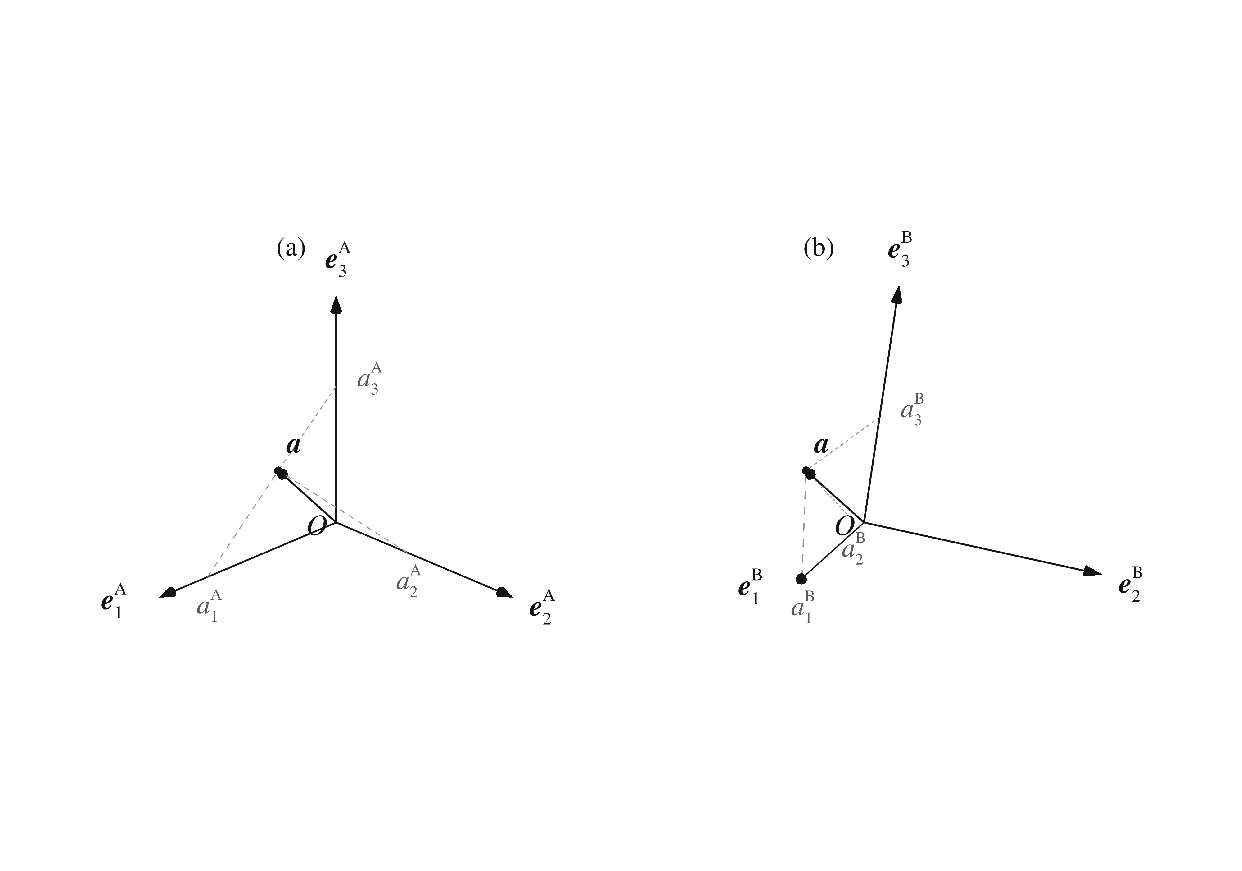
\includegraphics[trim={42.574bp 112.234bp 41.680bp 104.770bp},clip,width=.90\textwidth,height=.30\textheight,keepaspectratio]{figures/tecplot/concept_cambio-componentes.pdf}
\caption{Un mismo vector $\bm a$ expresado en las bases (a) $A$ y (b) $B$. Las líneas auxiliares muestran sus proyecciones. La transformación $\bm a^A=\bm Q_{AB}\bm a^B$ cambia las componentes y conserva el vector geométrico.}\label{fig:cambio-componentes}
\end{figure*}

\subsection{Sistemas de referencia y giro nominal}
El sistema newtoniano $\mathcal F_N=\{O_N;\bm E_1,\bm E_2,\bm E_3\}$ se considera inercial. El vector $\bm E_3$ es vertical, $\bm E_1$ apunta en la dirección del viento medio y $\bm E_2=\bm E_3\times\bm E_1$. El sistema de la base $\mathcal F_B$ tiene ejes paralelos a los de $N$ y origen $\bm c_B(t)=\bm c_{B0}+\bm u_g(t)$; $\bm u_g$ es la traslación prescrita del suelo. Por tanto, $\bm Q_{NB}=\I$, pero $B$ no es inercial cuando $\ddot{\bm u}_g\ne\bm0$.

El sistema $\mathcal F_G$ tiene origen en el punto de referencia de la góndola. Su orientación nominal coincide con la de $N$. El sistema $\mathcal F_H$ tiene origen sobre el eje del cubo y gira nominalmente respecto de $G$. Una barra superior distingue las orientaciones nominales de las orientaciones perturbadas. Así,

\begin{align}
\overline{\bm Q}_{NG}&=\I,\qquad
\overline{\bm Q}_{NH}(t)=\bm R_1(\psi(t)),\nonumber\\
\bm R_1(\psi)&=
\begin{bmatrix}1&0&0\\0&\cos\psi&-\sin\psi\\0&\sin\psi&\cos\psi\end{bmatrix},\nonumber\\
\psi(t)&=\psi_0+\Omega t,\qquad \Omega=\text{constante}.
\label{eq:rotacion-nominal}
\end{align}

El azimut $\psi$ se mide con la regla de la mano derecha alrededor de $\bm E_1$; $\psi_0$ es su valor inicial y $\Omega$ se expresa en radianes por segundo. No se incluye un movimiento nominal de orientación de la góndola para seguir cambios en la dirección del viento. Las pequeñas vibraciones de la góndola, del cubo y de la torre sí forman parte de la respuesta estructural.
La figura~\ref{fig:sistemas-globales} sitúa los orígenes y las tres direcciones de cada triedro en el espacio. La figura~\ref{fig:giro-nominal} muestra la rotación de los ejes del cubo respecto de los inerciales. El superíndice $H,n$ en los dibujos identifica la orientación nominal representada con una barra superior en el texto.

\begin{figure*}[tp]
\centering
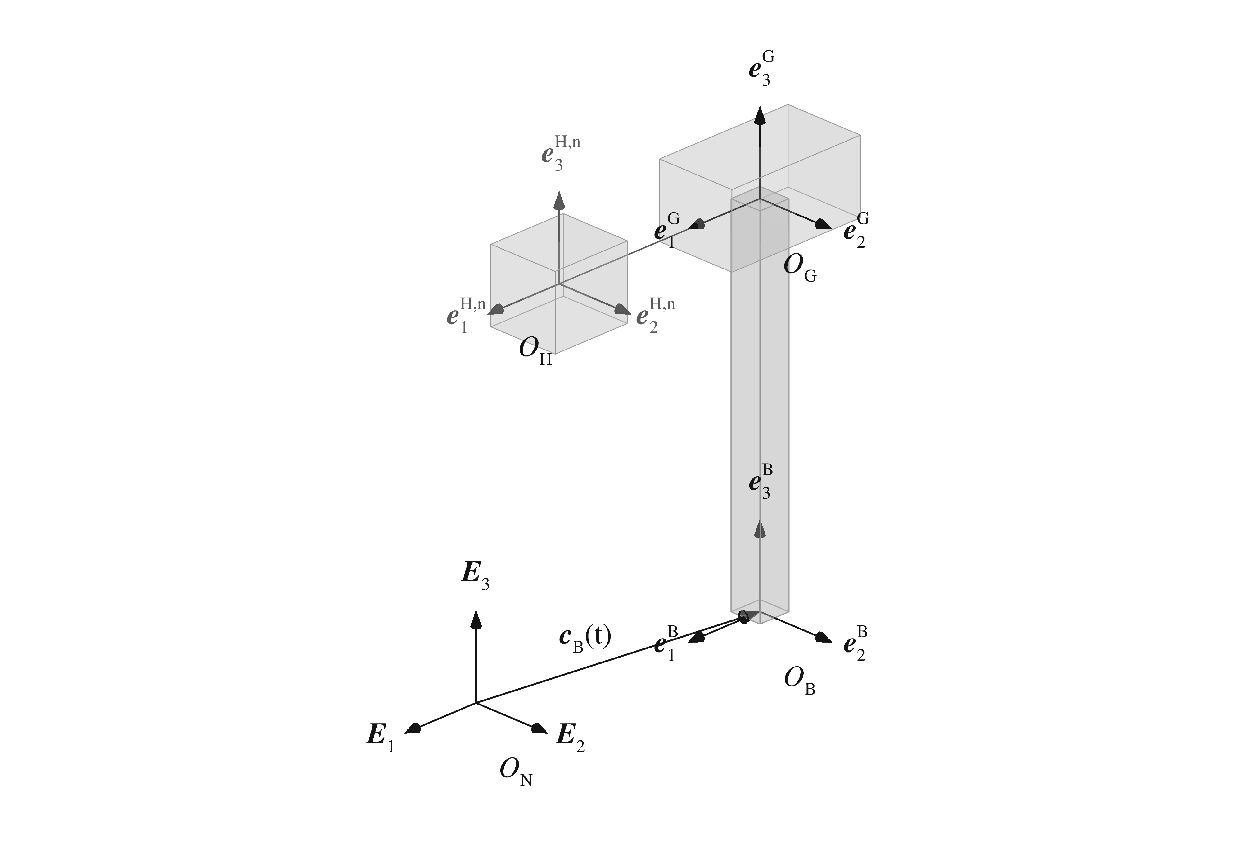
\includegraphics[trim={169.820bp 26.585bp 172.651bp 18.065bp},clip,width=.83\textwidth,height=.35\textheight,keepaspectratio]{figures/tecplot/concept_sistemas-lateral.pdf}
\caption{Orígenes y triedros de referencia en una vista espacial, con azimut nominal nulo. Los ejes de $B$ y $G$ son paralelos a los inerciales; $\bm c_B(t)$ localiza la base. El superíndice $H,n$ identifica el triedro nominal del cubo. Las separaciones y los volúmenes son esquemáticos.}\label{fig:sistemas-globales}
\end{figure*}

\begin{figure*}[tp]
\centering
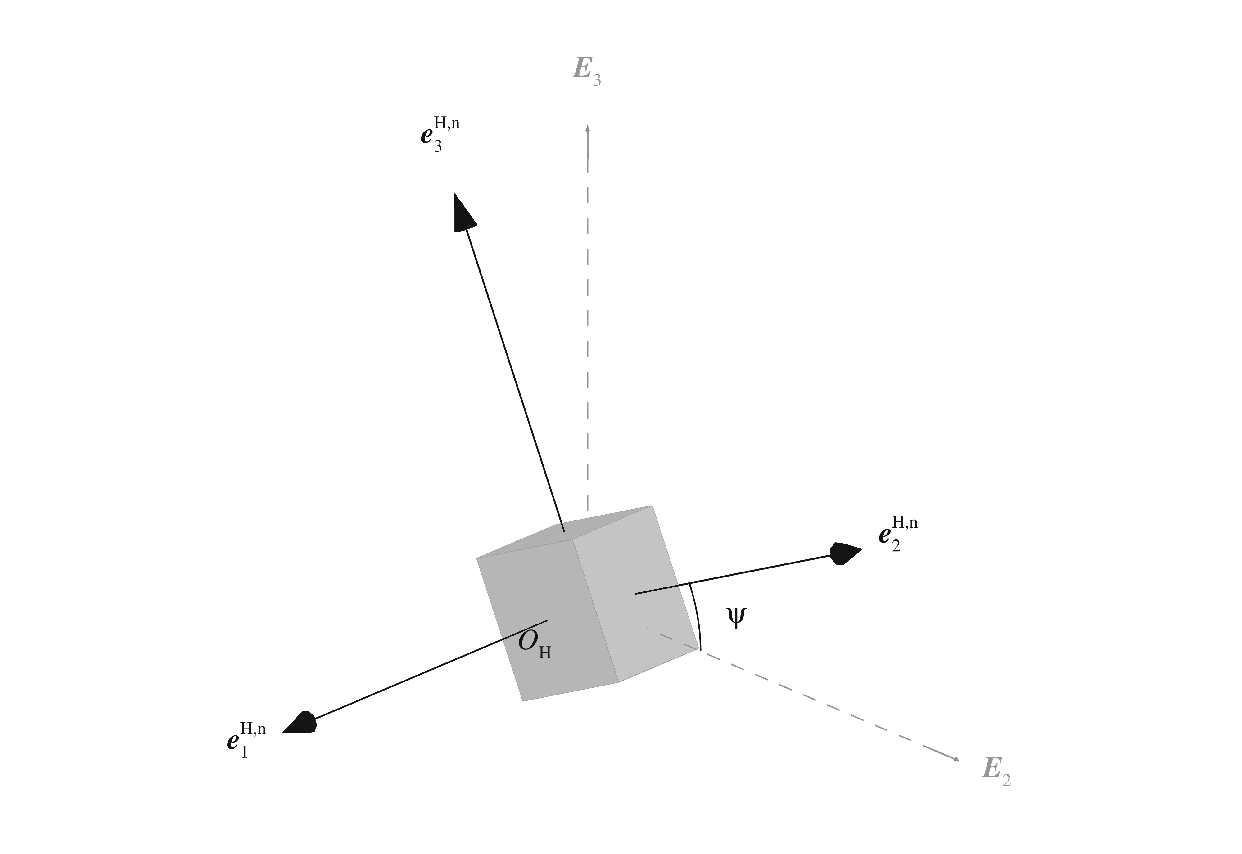
\includegraphics[trim={103.068bp 26.585bp 104.707bp 21.353bp},clip,width=.70\textwidth,height=.29\textheight,keepaspectratio]{figures/tecplot/concept_cubo-nominal.pdf}
\caption{Rotación nominal del cubo alrededor del eje 1 común. Los ejes inerciales 2 y 3 son discontinuos; los nominales $H,n$ son continuos. El arco $\psi$ sigue la regla de la mano derecha. La orientación nominal puede ser grande, independientemente de las pequeñas rotaciones estructurales.}\label{fig:giro-nominal}
\end{figure*}

Cada pala $b=1,2,3$ tiene un sistema $\mathcal F_{P_b}$ en su raíz. Su eje 1 es longitudinal, el eje 2 es tangencial al rotor y el eje 3 es normal al plano del rotor. Para palas equiespaciadas, sin cono ni paso inicial, se define

\begin{align}
\beta_b&=\frac{2\pi(b-1)}3,\qquad
\bm Q_{\rm mont}=
\begin{bmatrix}0&0&1\\0&-1&0\\1&0&0\end{bmatrix},\nonumber\\
\bm Q_{HP_b}&=\bm R_1(\beta_b)\bm Q_{\rm mont},\nonumber\\
\overline{\bm Q}_{NP_b}(t)
&=\overline{\bm Q}_{NH}(t)\bm Q_{HP_b}.
\label{eq:marcos-palas}
\end{align}

La primera columna de $\bm Q_{HP_b}$ es la dirección radial
$\bm d_{1b}^H=[0,-\sin\beta_b,\cos\beta_b]^\tr$.
La segunda es $\bm d_{2b}^H=[0,-\cos\beta_b,-\sin\beta_b]^\tr$ y la tercera es $\bm d_{3b}^H=[1,0,0]^\tr$. La pala 1 apunta hacia arriba cuando $\psi=0$. Si $r_h$ es la distancia del origen del cubo a la raíz, su posición nominal es

\begin{equation}
\overline{\bm c}_{P_b}^N
=\overline{\bm c}_H^N+\overline{\bm Q}_{NH}\bm r_{b0},
\qquad \bm r_{b0}=r_h\bm d_{1b}^H.
\label{eq:raices}
\end{equation}

Un ángulo de paso fijo $\alpha_b$ se introduce multiplicando $\bm Q_{HP_b}$ por $\bm R_1(\alpha_b)$ a la derecha, pues corresponde a una rotación alrededor del eje longitudinal de la pala. No se confunde este montaje con el azimut ni con la torsión elástica.
La figura~\ref{fig:marcos} particulariza las bases de las tres raíces al azimut cero. El índice inicial de $\bm d_{ib}$ identifica el eje y el segundo identifica la pala.

\begin{figure*}[tp]
\centering
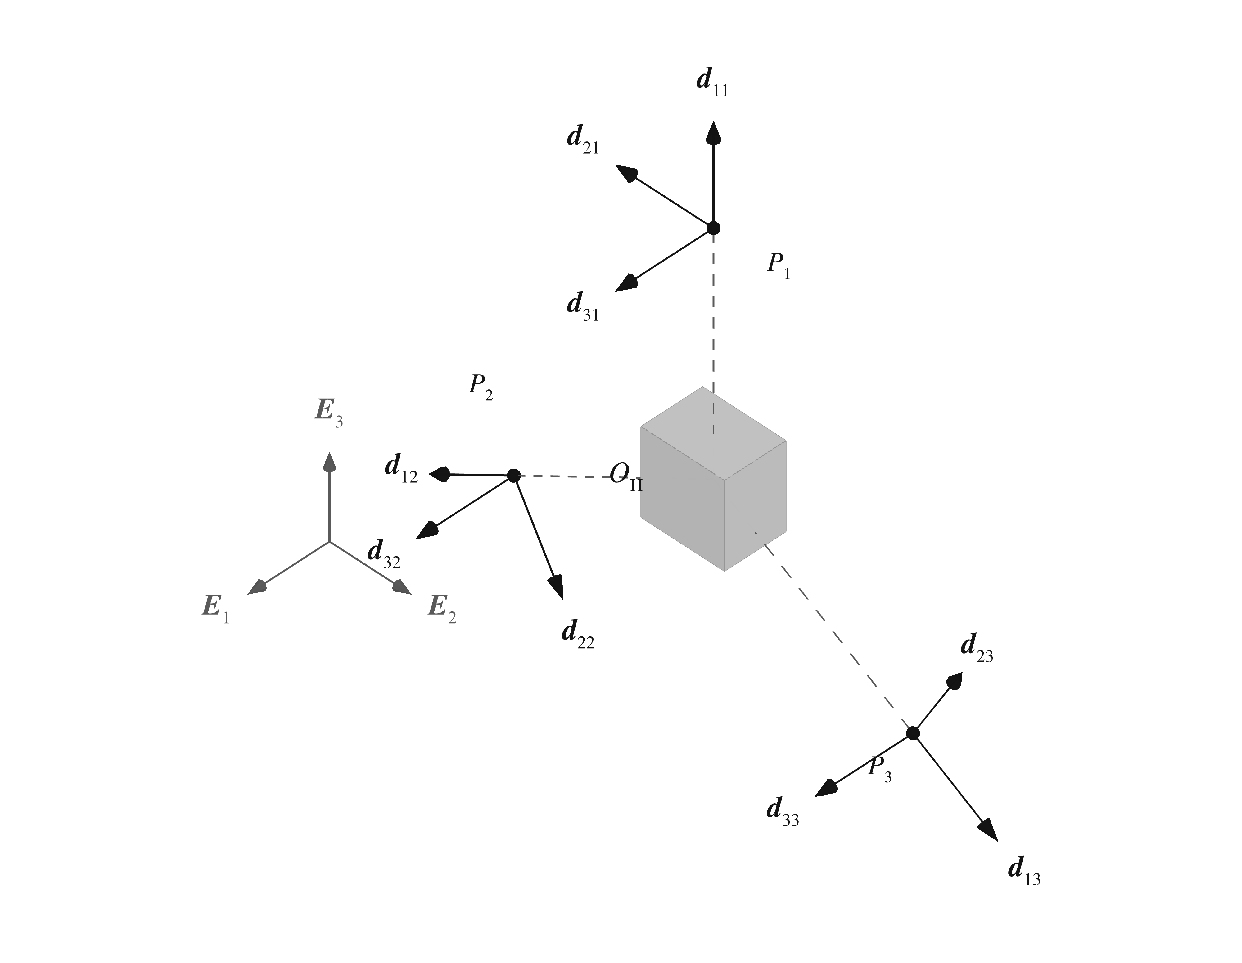
\includegraphics[trim={90.701bp 31.277bp 90.701bp 25.738bp},clip,width=.83\textwidth,height=.37\textheight,keepaspectratio]{figures/tecplot/concept_marcos.pdf}
\caption{Triedros de las tres raíces para $\psi=0$. El director $\bm d_{1b}$ es longitudinal, $\bm d_{2b}$ es tangencial y $\bm d_{3b}=\bm E_1$ completa la base dextrógira. Las raíces $P_b$ están separadas $120^\circ$ alrededor de $O_H$.}\label{fig:marcos}
\end{figure*}

El giro de la ecuación~\eqref{eq:rotacion-nominal} es una operación prescrita: se proporciona al modelo, en lugar de calcularse a partir de un balance del accionamiento. Se prescribe la rotación nominal y se conserva como incógnita la pequeña torsión relativa de la conexión. Si se impusiera exactamente la velocidad instantánea del cubo, habría que restringir también esa coordenada. La torre y la góndola no giran nominalmente con el rotor; sus desplazamientos se deben a la excitación de base y a las deformaciones estructurales.

\subsection{Cinemática continua de los componentes}
La posición de una partícula de un cuerpo rígido se escribe

\begin{equation}
\bm x(\bm\rho,t)=\bm c(t)+\bm Q(t)\bm\rho,
\label{eq:cuerpo-rigido}
\end{equation}

donde $\bm c$ es la posición de su punto de referencia y $\bm\rho$ es el vector material constante desde dicho punto. La matriz $\bm Q$ transforma componentes de la base solidaria con el cuerpo a la base inercial. Para un cuerpo deformable de tipo viga, el origen y la orientación de la sección dependen además de la coordenada longitudinal material $S$:

\begin{align}
\bm X(S,\xi_2,\xi_3)
&=\bm R(S)+\xi_2\bm D_2(S)+\xi_3\bm D_3(S),\nonumber\\
\bm x(S,\xi_2,\xi_3,t)
&=\bm r(S,t)+\xi_2\bm d_2(S,t)+\xi_3\bm d_3(S,t).
\label{eq:viga-continua}
\end{align}

Aquí $\bm R$ y $\bm r$ son las líneas de referencia y actual; $\xi_2,\xi_3$ localizan la misma partícula dentro de la sección en ambas configuraciones. Los directores $\bm D_i$ y $\bm d_i$ forman bases ortonormales de referencia y actual, respectivamente. Las secciones permanecen planas y rígidas en su propio plano, pero su normal $\bm d_1=\bm d_2\times\bm d_3$ puede no coincidir con la tangente de $\bm r$. Esta independencia permite representar la deformación por cortante de la teoría de Timoshenko. No se resuelve un campo adicional de alabeo; su efecto torsional se incorpora mediante una rigidez equivalente.

La figura~\ref{fig:viga} localiza una partícula mediante la línea de referencia y los directores de la sección. La figura~\ref{fig:cortante} distingue la normal seccional de la tangente, haciendo explícita su independencia cinemática.

\begin{figure*}[tp]
\centering
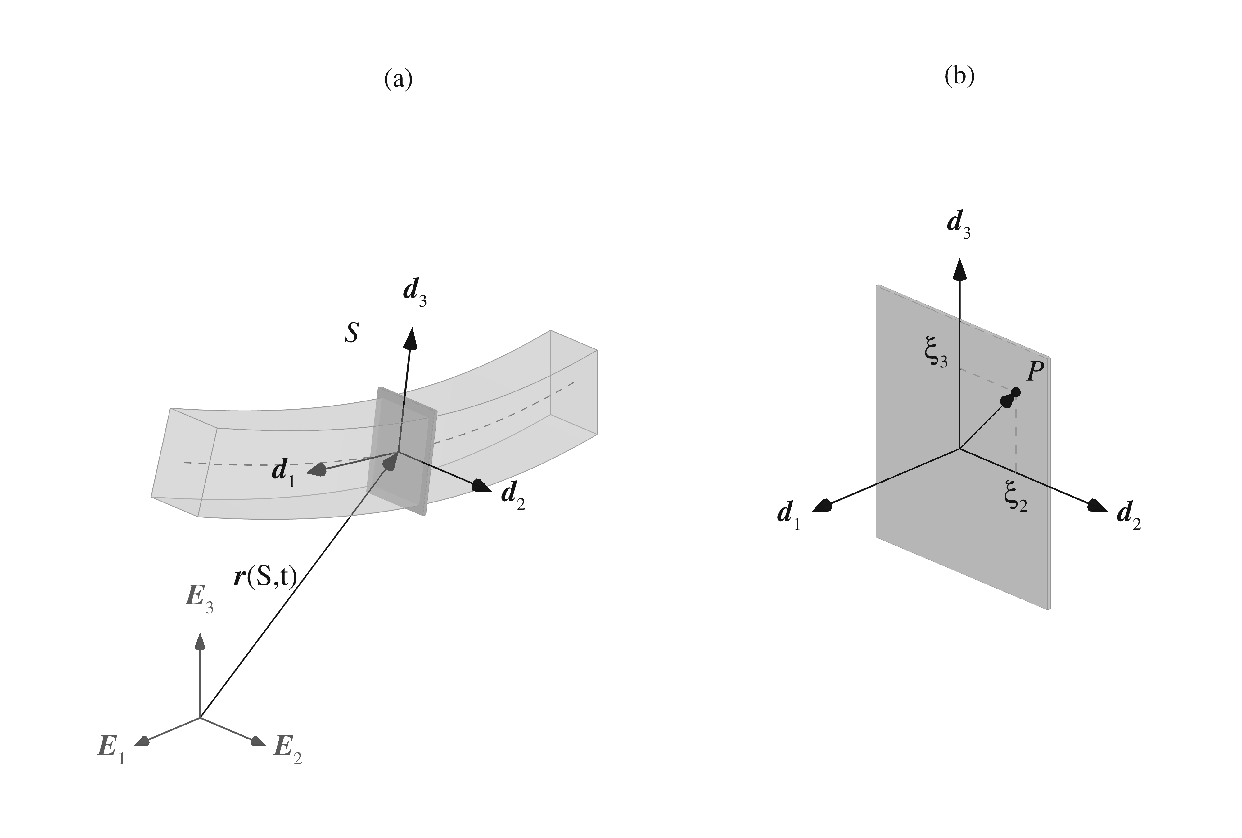
\includegraphics[trim={40.488bp 29.471bp 42.276bp 24.831bp},clip,width=.96\textwidth,height=.34\textheight,keepaspectratio]{figures/tecplot/concept_particula-seccion.pdf}
\caption{Posición de una partícula de viga: (a) línea $\bm r(S,t)$ y orientación de la sección; (b) detalle de la sección, donde $\bm x_P=\bm r+\xi_2\bm d_2+\xi_3\bm d_3$. La envolvente transparente permite ver la línea de referencia; sus superficies no añaden grados de libertad.}\label{fig:viga}
\end{figure*}

\begin{figure*}[tp]
\centering
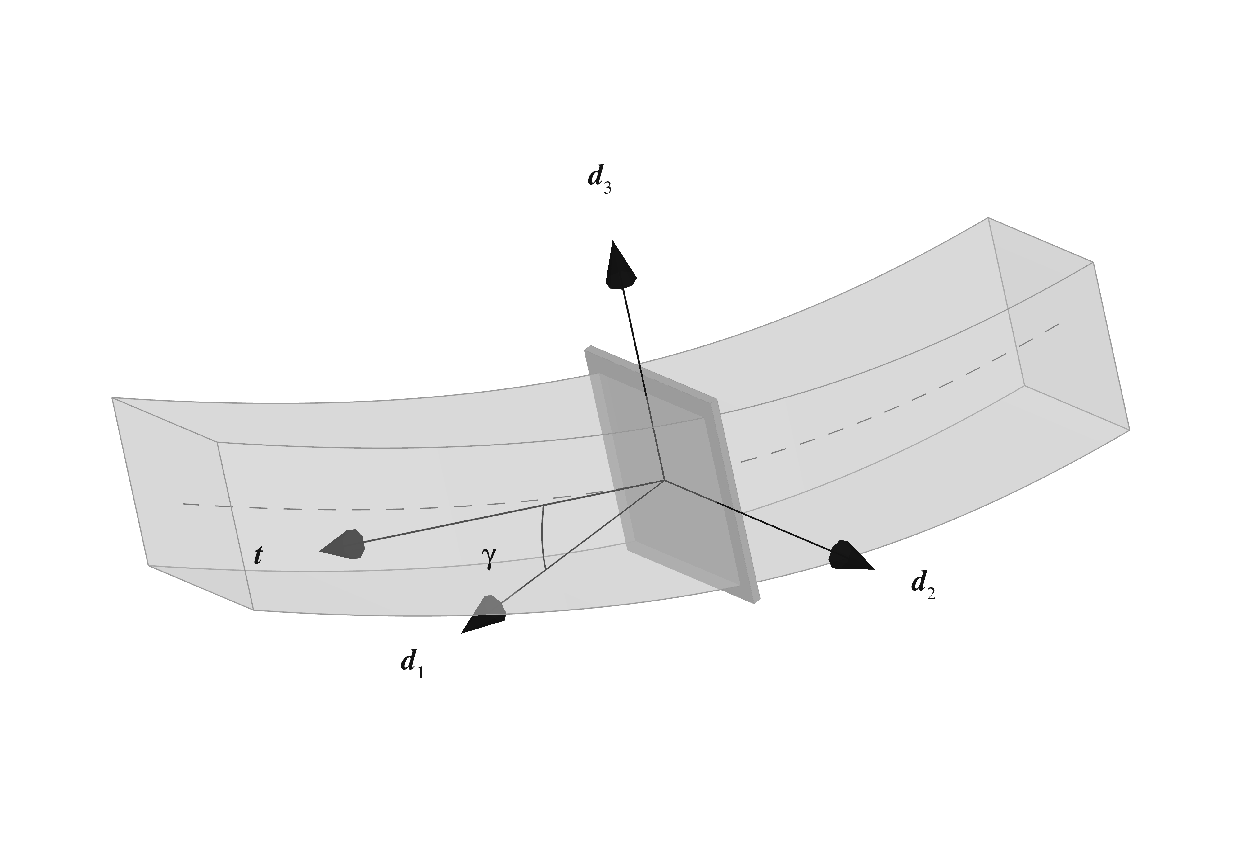
\includegraphics[trim={47.342bp 78.302bp 47.342bp 72.622bp},clip,width=.82\textwidth,height=.32\textheight,keepaspectratio]{figures/tecplot/concept_shear.pdf}
\caption{Independencia entre la normal seccional $\bm d_1$ y la tangente $\bm t$ a la línea de referencia. El ángulo $\gamma$ ilustra el cortante en el plano del dibujo; es una componente angular ilustrativa, no el vector completo de deformaciones $\bm\gamma$ de la ecuación~\eqref{eq:medidas-viga}.}\label{fig:cortante}
\end{figure*}

En una pala recta, la posición nominal de la línea se obtiene sumando a la ecuación~\eqref{eq:raices} el vector $\overline{\bm Q}_{NP_b}[S,0,0]^\tr$. En la torre se toma $S$ desde la base hacia la góndola y la terna nominal $(\bm E_3,\bm E_1,\bm E_2)$. Así queda definida la relación entre las coordenadas materiales de cada viga y la geometría de la máquina.

La rotación de perturbación se representa mediante
$\bm E(\bm\theta)=\exp(\Sx{\theta})$.
Para la góndola y el cubo, $\bm Q=\overline{\bm Q}\bm E$; para una sección, la misma relación se aplica después de incluir su orientación de montaje. El vector $\bm\theta$ expresa el incremento angular en la base nominal correspondiente. No es, en general, un vector de ángulos de Euler, ni su derivada coincide exactamente con la velocidad angular. Esa relación se especifica al deducir los términos inerciales.

La figura~\ref{fig:configuraciones} compara la referencia material con el movimiento nominal y con el movimiento perturbado. Se denota por $\overline{\bm x}(\bm X,t)$ la posición que tendría una partícula bajo el movimiento nominal y por $\overline{\mathcal B}_t$ la configuración correspondiente. La diferencia $\bm x-\overline{\bm x}$ es su desplazamiento respecto de esa trayectoria; en una viga incluye tanto la traslación del origen seccional como la variación de orientación de la sección.

\begin{figure*}[tp]
\centering
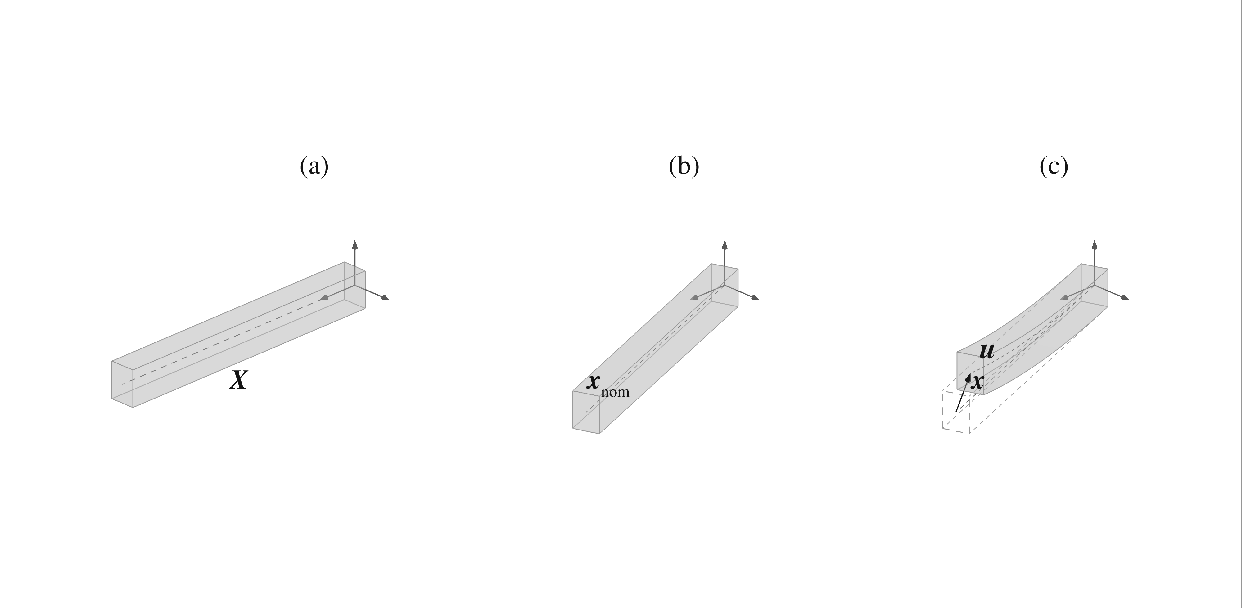
\includegraphics[trim={47.491bp 0.000bp 0.000bp 0.000bp},clip,width=.98\textwidth,height=.24\textheight,keepaspectratio]{figures/tecplot/concept_tresniveles.pdf}
\caption{Una misma porción material en (a) referencia, (b) movimiento nominal y (c) configuración perturbada. En (c), el contorno discontinuo reproduce la configuración nominal y la flecha $\bm u$ señala la diferencia en el extremo. $\bm x_{\rm nom}$ representa $\overline{\bm x}$; los desplazamientos están ampliados para distinguir los estados.}\label{fig:configuraciones}
\end{figure*}

La deformación se mide respecto de la geometría material, no del observador. Por ejemplo, si $\bm Q_s=[\bm d_1,\bm d_2,\bm d_3]$ y $\bm Q_{s0}=[\bm D_1,\bm D_2,\bm D_3]$, las medidas de extensión--cortante y de curvatura--torsión son

\begin{align}
\bm\gamma&=\bm Q_s^\tr\bm r'-\bm Q_{s0}^\tr\bm R',\nonumber\\
\bm\kappa&=\operatorname{axial}(\bm Q_s^\tr\bm Q_s')
-\operatorname{axial}(\bm Q_{s0}^\tr\bm Q_{s0}').
\label{eq:medidas-viga}
\end{align}

La prima indica derivación respecto de $S$ y $\operatorname{axial}([\bm a]_\times)=\bm a$. Un movimiento rígido superpuesto no altera estas medidas. Para una viga inicialmente recta se utilizará su aproximación lineal en los desplazamientos y giros estructurales; la rotación nominal se conserva por separado.

\subsection{Estado de operación y perturbaciones}
Se distinguen la geometría material $\mathcal B_0$, la trayectoria nominal impuesta y la configuración estructural de equilibrio $\bm q_0$. Esta última depende de las cargas, de la velocidad de giro y de las propiedades de los componentes. Las coordenadas estructurales se escriben como $\bm q(t)=\bm q_0+\delta\bm q(t)$; $\delta\bm q$ describe las vibraciones y no incluye de nuevo el azimut prescrito.

Cuando cargas y coeficientes son estacionarios en las coordenadas escogidas, $\bm q_0$ define un equilibrio relativo: la deformación es constante en ellas, aunque las partículas del rotor sigan moviéndose. Una gravedad fija en el sistema inercial o un flujo no uniforme pueden impedir esta estacionariedad. En ese caso, el equilibrio a un azimut dado y su linealización constituyen una aproximación local, no una solución periódica completa. Se conservan las propiedades de masa de referencia; la precarga modifica la rigidez tangente dentro de la hipótesis de pequeñas deformaciones.

\FloatBarrier
\section{Propiedades seccionales y masa}
\subsection{Momentos geométricos y másicos}
Las propiedades se definen en una sección material $A_0(S)$, utilizando la densidad de referencia $\rho_0$ y coordenadas locales $y,z$. El tensor geométrico de segundo momento respecto del centro geométrico es

\begin{equation}
\bm I_A=\int_{A_0}
\big[(\bm\xi\cdot\bm\xi)\I-\bm\xi\otimes\bm\xi\big]\,\dd A,
\qquad \bm\xi=[0,y,z]^\tr.
\end{equation}

De él se obtienen $I_y=\int_{A_0}z^2\dd A$, $I_z=\int_{A_0}y^2\dd A$ y el momento polar $I_y+I_z$. El área es $A=\int_{A_0}\dd A$. En ejes principales y para una sección sin acoplamientos constitutivos, la matriz de rigidez seccional es

\begin{equation}
\bm K_s=\operatorname{diag}(EA,GA_{sy},GA_{sz},GJ_t,EI_y,EI_z),
\label{eq:Ks}
\end{equation}

donde $E$ es el módulo de Young, $G$ es el módulo de corte, $A_{sy},A_{sz}$ son las áreas efectivas de cortante y $J_t$ es la constante torsional. Las áreas efectivas ya incluyen la corrección por la distribución de tensiones de corte. Los momentos $I_y,I_z$ y $J_t$ tienen unidades de $\mathrm{m^4}$, pero $J_t$ no coincide en general con $I_y+I_z$. La matriz relaciona las deformaciones generalizadas con las resultantes conjugadas:

\begin{equation}
\begin{bmatrix}\bm n\\\bm m_s\end{bmatrix}
=\bm K_s\begin{bmatrix}\bm\gamma\\\bm\kappa\end{bmatrix}.
\label{eq:constitutiva}
\end{equation}

Las componentes de $\bm n$ son la fuerza axial y las dos fuerzas de corte; las de $\bm m_s$ son el momento torsor y los dos momentos flectores. Se obtienen integrando la tracción seccional $\bm t$ y su momento: $\bm n=\int_{A_0}\bm t\,\dd A$ y $\bm m_s=\int_{A_0}\bm\xi\times\bm t\,\dd A$, en la aproximación de pequeñas deformaciones. Su trabajo por unidad de longitud es $\bm n\cdot\delta\bm\gamma+\bm m_s\cdot\delta\bm\kappa$. Una sección compuesta o excéntrica puede requerir una matriz constitutiva simétrica completa; la expresión diagonal~\eqref{eq:Ks} supone que esos acoplamientos son despreciables.

Para las propiedades de masa se utiliza el centro de masa seccional $C$, que no tiene por qué coincidir con el centro geométrico. Si $\bm\rho_C$ une $C$ con una partícula de la sección,

\begin{align}
\mu&=\int_{A_0}\rho_0\,\dd A,\qquad
\int_{A_0}\rho_0\bm\rho_C\,\dd A=\bm0,\nonumber\\
\bm j_C&=\int_{A_0}\rho_0
\big[(\bm\rho_C\cdot\bm\rho_C)\I-\bm\rho_C\otimes\bm\rho_C\big]\,\dd A.
\label{eq:sectioninertia}
\end{align}

En ejes principales centroidales, $j_y=\int_{A_0}\rho_0 z^2\dd A$, $j_z=\int_{A_0}\rho_0 y^2\dd A$ y $j_x=j_y+j_z$ para una sección plana. Las unidades de $\mu$ y $\bm j_C$ son $\mathrm{kg/m}$ y $\mathrm{kg\,m}$. Los elementos no diagonales son los negativos de las integrales de los productos de coordenadas. Así se distingue un tensor de inercia másico de un segundo momento geométrico de área.

Para un material homogéneo e isótropo, $G=E/[2(1+\nu)]$, donde $\nu$ es el coeficiente de Poisson; además, $\mu=\rho_0 A$ y $\bm j_C=\rho_0\operatorname{diag}(I_y+I_z,I_y,I_z)$. En las palas, las rigideces y las propiedades de masa pueden proceder directamente de un análisis seccional. Si una distribución tabulada debe normalizarse a una masa total conocida $m_b^\star$, manteniendo su forma espacial y sus radios de giro, se emplea

\begin{equation}
c_b=\frac{m_b^\star}{\int_0^{L_b}\mu^{\rm tab}(S)\,\dd S},
\qquad (\mu,\bm j_C)=c_b(\mu^{\rm tab},\bm j_C^{\rm tab}).
\label{eq:massscale}
\end{equation}

Aquí $L_b$ es la longitud de la pala y el superíndice $\mathrm{tab}$ identifica los datos de partida. El factor $c_b$ es adimensional y se aplica al tensor completo. Esta normalización no determina excentricidades ni productos de inercia ausentes en los datos. Suponerlos nulos constituye una idealización adicional que debe ser compatible con los ejes seccionales adoptados.

\subsection{Matriz espacial de masa}
Sea $\bm r_C$ el vector desde el origen de la sección hasta su centro de masa, expresado en la misma base que las velocidades. La velocidad centroidal es $\bm v_C=\bm v_O+\bm\omega_s\times\bm r_C$, donde $\bm v_O$ y $\bm\omega_s$ son la velocidad del origen y la velocidad angular de la sección. Al integrar la energía de sus partículas, la condición centroidal anula el término cruzado respecto de $C$ y se obtiene

\begin{equation}
\mathcal T_s=\tfrac12\mu\|\bm v_C\|^2
+\tfrac12\bm\omega_s^\tr\bm j_C\bm\omega_s.
\label{eq:energia-seccion}
\end{equation}

La figura~\ref{fig:masa-seccional} distingue el origen de la línea de referencia, el centro de masa y la posición de una partícula. El vector $\bm r_C+\bm\rho_C$ localiza la partícula desde el origen; el tensor $\bm j_C$ de la ecuación~\eqref{eq:sectioninertia}, en cambio, se calcula con distancias medidas desde $C$.

\begin{figure*}[tp]
\centering
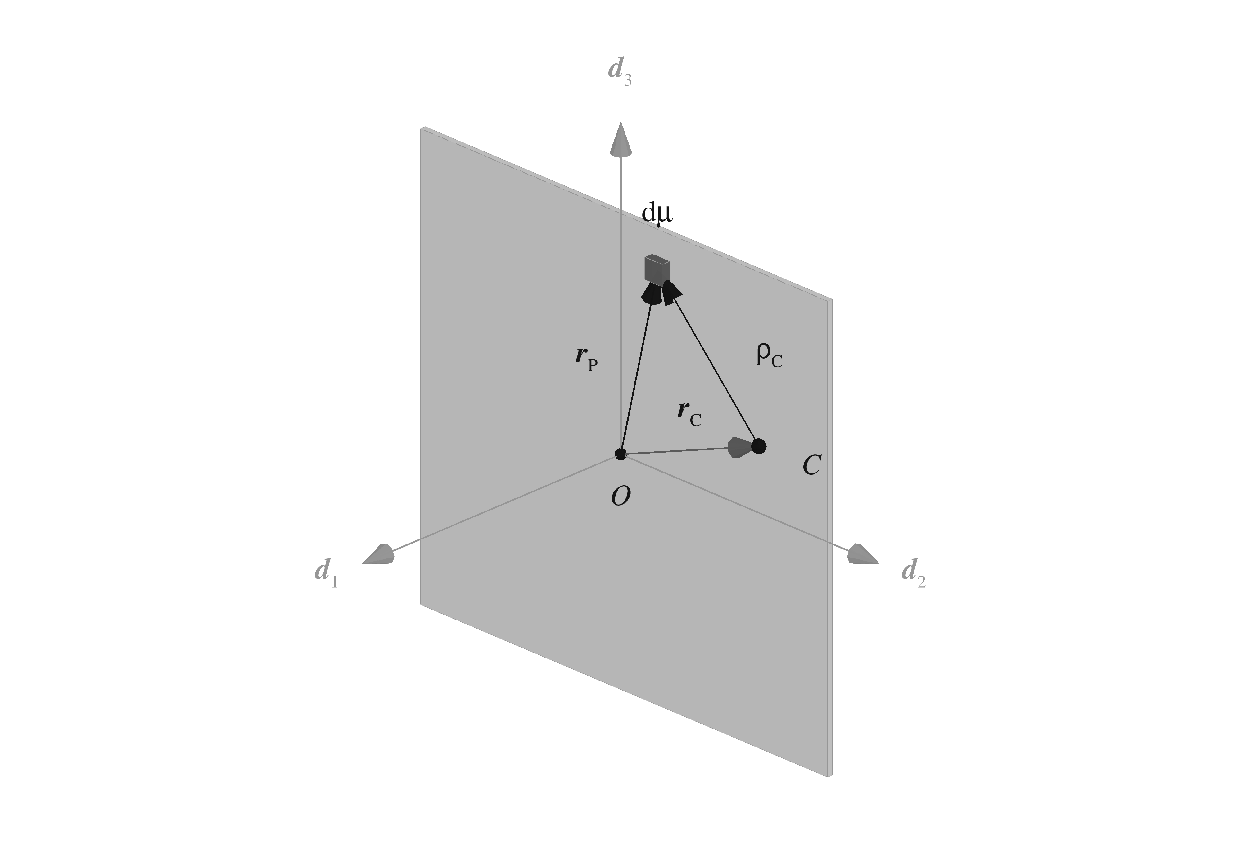
\includegraphics[trim={145.086bp 30.620bp 145.682bp 21.054bp},clip,width=.76\textwidth,height=.30\textheight,keepaspectratio]{figures/tecplot/paper_masa_seccional.pdf}
\caption{Geometría de la integración de masa: origen seccional $O$, centro de masa $C$ y contribución $\dd\mu=\rho_0\dd A$. La posición de la partícula satisface $\bm r_P=\bm r_C+\bm\rho_C$. La inercia centroidal usa $\bm\rho_C$; su traslado al origen utiliza $\bm r_C$. El espesor de la sección es ilustrativo.}\label{fig:masa-seccional}
\end{figure*}

Para expresar esta energía con respecto al origen seccional se introducen

\begin{equation}
\bm B_C=[\I,-\Sx{r_C}],\qquad \bm E_\theta=[\bm0,\I].
\end{equation}

En una referencia estacionaria y al primer orden cinemático,
$[\bm v_O^\tr,\bm\omega_s^\tr]^\tr=\dot{\bm\eta}$,
con $\bm\eta=[\bm u^\tr,\bm\theta^\tr]^\tr$. Entonces la parte cuadrática de la energía es

\begin{equation}
\mathcal T_s=\tfrac12\mu\|\bm B_C\dot{\bm\eta}\|^2
+\tfrac12(\bm E_\theta\dot{\bm\eta})^\tr\bm j_C(\bm E_\theta\dot{\bm\eta}),
\end{equation}

La matriz que multiplica estas velocidades generalizadas es, por tanto,

\begin{equation}
\bm M_s=\begin{bmatrix}
\mu\I&-\mu\Sx{r_C}\\
\mu\Sx{r_C}&\bm j_C-\mu\Sx{r_C}^2
\end{bmatrix}.
\label{eq:Ms}
\end{equation}

El bloque $-\mu\Sx{r_C}^2=\mu[(\bm r_C\cdot\bm r_C)\I-\bm r_C\otimes\bm r_C]$ corresponde al teorema de ejes paralelos. Los bloques cruzados representan el acoplamiento entre traslación y rotación debido a la excentricidad. Durante el giro nominal, la energía contiene términos adicionales, que se deducen en lugar de identificar la velocidad angular total con $\dot{\bm\theta}$.

Para un cuerpo rígido se sustituye $\mu$ por $m=\int_{\mathcal B_0}\rho_0\,\dd V$ y $\bm j_C$ por $\bm J_C=\int_{\mathcal B_0}\rho_0[(\bm\rho_C\cdot\bm\rho_C)\I-\bm\rho_C\otimes\bm\rho_C]\,\dd V$, con unidades de $\mathrm{kg\,m^2}$. La transformación~\eqref{eq:cambio-base} sitúa el tensor en la base de ensamblaje y el teorema de ejes paralelos lo refiere al punto elegido en la góndola o el cubo. La orientación y la excentricidad actúan sobre el tensor completo, no solo sobre sus entradas diagonales.

\section{Discretización estructural}
\label{sec:elementos}
\subsection{Variables nodales e interpolación}
La línea de referencia de cada viga se divide en elementos de dos nodos. Cada nodo posee tres desplazamientos y tres rotaciones estructurales, de modo que
$\bm q_i=[\bm u_i^\tr,\bm\theta_i^\tr]^\tr$ y cada elemento tiene doce coordenadas antes de aplicar restricciones. La coordenada local $x\in[0,L]$ recorre la longitud de referencia del elemento; corresponde a un intervalo de la coordenada material $S$. Los ejes locales $x,y,z$ coinciden con los ejes 1, 2 y 3 de la sección. En ellos, el campo
$\bm\eta=[u,v,w,\theta_x,\theta_y,\theta_z]^\tr$
produce, al linealizar la ecuación~\eqref{eq:medidas-viga},

\begin{equation}
\bm\varepsilon=[u',v'-\theta_z,w'+\theta_y,
\theta_x',\theta_y',\theta_z']^\tr.
\end{equation}

Las tres primeras componentes son extensión y cortantes; las tres últimas son torsión y curvaturas. La prima indica aquí derivación respecto de $x$. Se interpola $\bm\eta=\bm N(x)\bm q_e^\ell$, donde $\bm N$ es de tamaño $6\times12$ y $\ell$ identifica componentes locales. Al sustituir la interpolación en las relaciones de deformación se obtiene $\bm\varepsilon=\bm B(x)\bm q_e^\ell$. Por el trabajo virtual interno y la energía cinética, las matrices elementales son

\begin{align}
U_e&=\tfrac12\int_0^L\bm\varepsilon^\tr\bm K_s\bm\varepsilon\,\dd x,\nonumber\\
\bm K_e^\ell&=\int_0^L\bm B^\tr\bm K_s\bm B\,\dd x,\nonumber\\
\bm M_e^\ell&=\int_0^L\bm N^\tr\bm M_s\bm N\,\dd x.
\label{eq:elementenergy}
\end{align}

Se utiliza una interpolación cerrada de dos nodos para propiedades desacopladas constantes por elemento \citep{reddy2006}. Los bloques de rigidez y las funciones utilizadas por la masa se detallan en el Apéndice A. El límite $GA_s\to\infty$ elimina la deformación de cortante; si se conserva la inercia rotacional, el modelo dinámico límite es de tipo Rayleigh, no Euler--Bernoulli clásico.

\subsection{Orientación y ensamblaje}
Las posiciones de referencia $\bm X_I,\bm X_J$ de los extremos y un punto auxiliar $\bm X_a$ determinan la base del elemento:

\begin{align}
L&=\|\bm X_J-\bm X_I\|,\quad
\bm e_1=(\bm X_J-\bm X_I)/L,\nonumber\\
\bm p&=(\I-\bm e_1\bm e_1^\tr)(\bm X_a-\bm X_I),\nonumber\\
\bm e_3&=\bm p/\|\bm p\|,\qquad
\bm e_2=\bm e_3\times\bm e_1.
\label{eq:base-elemento}
\end{align}

El punto auxiliar debe estar fuera del eje y se elige para reproducir las direcciones seccionales de montaje. Con $\bm Q_e=[\bm e_1,\bm e_2,\bm e_3]$ y $\bm R_e=\bm Q_e^\tr$,

\begin{equation}
\bm q_e^\ell=\bm T_e\bm q_e^g,\qquad
\bm T_e=\operatorname{diag}(\bm R_e,\bm R_e,\bm R_e,\bm R_e).
\end{equation}

El superíndice $g$ identifica componentes en los ejes de ensamblaje, paralelos a los de $N$ para la geometría considerada. El símbolo $\operatorname{diag}$ con argumentos matriciales indica una matriz diagonal por bloques. La conservación del trabajo virtual da $\bm K_e^g=\bm T_e^\tr\bm K_e^\ell\bm T_e$ y $\bm M_e^g=\bm T_e^\tr\bm M_e^\ell\bm T_e$. Esta transformación en una configuración dada no reemplaza la transformación temporal de velocidades y aceleraciones.

La figura~\ref{fig:elemento} identifica los extremos del elemento y la dirección auxiliar proyectada que construye su base espacial. El punto auxiliar solo fija los ejes transversales; no es un nodo con grados de libertad.

\begin{figure*}[tp]
\centering
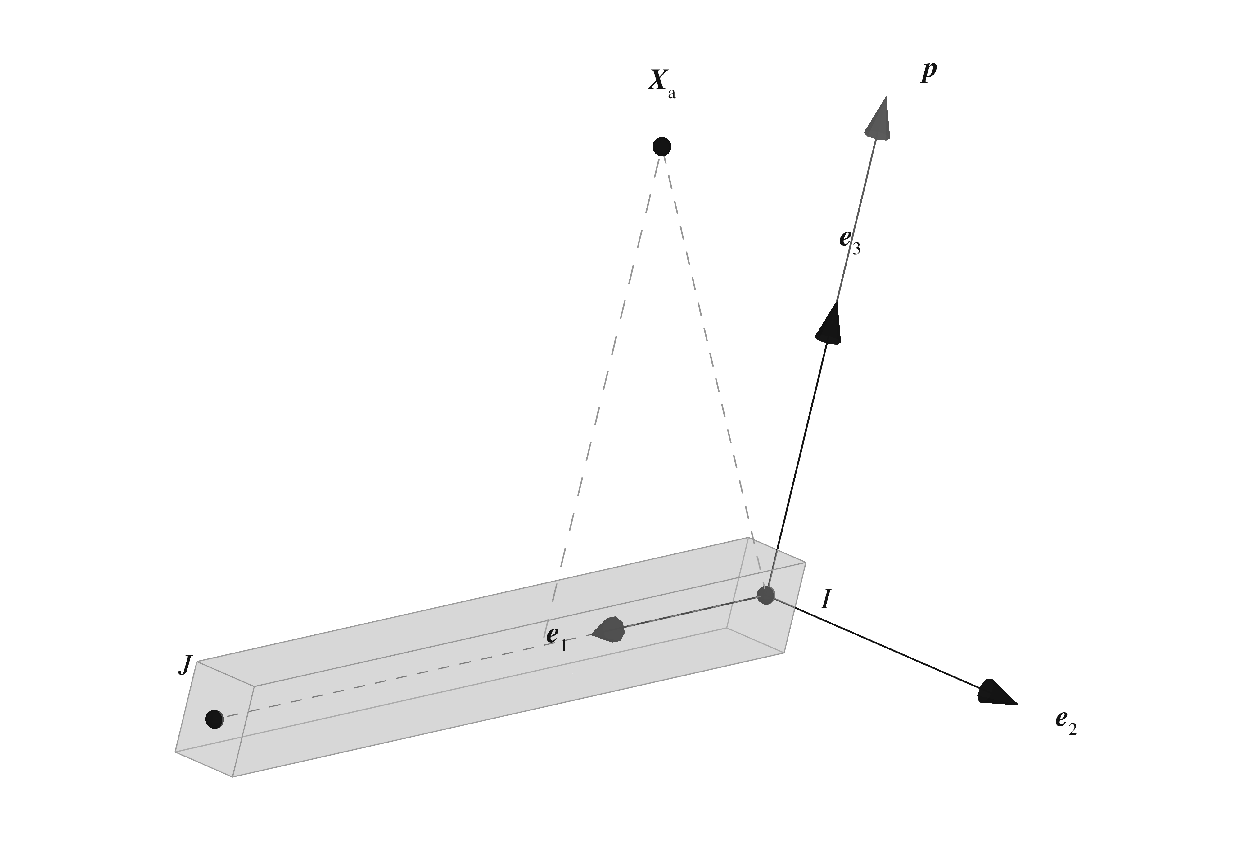
\includegraphics[trim={77.738bp 30.620bp 72.970bp 24.343bp},clip,width=.82\textwidth,height=.32\textheight,keepaspectratio]{figures/tecplot/concept_elemento.pdf}
\caption{Orientación de un elemento entre $I$ y $J$. El eje $\bm e_1$ sigue la cuerda; la proyección $\bm p$ del punto auxiliar $\bm X_a$ sobre el plano normal determina $\bm e_3$. Se completa el triedro con $\bm e_2=\bm e_3\times\bm e_1$. El punto auxiliar no es un nodo estructural.}\label{fig:elemento}
\end{figure*}

Si $\bm L_e$ extrae de $\bm q$ las coordenadas del elemento, el ensamblaje de una matriz genérica $\bm A$, que puede ser de masa o rigidez, sigue

\begin{equation}
\bm A=\sum_e\bm L_e^\tr\bm A_e^g\bm L_e
+\sum_R\bm L_R^\tr\bm A_R^g\bm L_R,
\end{equation}

donde $\bm L_R$ ubica las contribuciones de cuerpos rígidos y conexiones en las coordenadas globales. Los vínculos cinemáticos se imponen después de este ensamblaje, por lo que todavía se conservan las coordenadas de ambos lados de cada unión.

\subsection{Conexión entre góndola y cubo}
Los puntos de referencia de la góndola $G$ y del cubo $H$ se separan nominalmente por $\bm d=\overline{\bm c}_H-\overline{\bm c}_G$. En una misma base, la deformación relativa de la conexión es

\begin{equation}
\bm\Delta_d=\begin{bmatrix}
\bm u_H-\bm u_G+\Sx{d}\bm\theta_G\\
\bm\theta_H-\bm\theta_G
\end{bmatrix}=\bm B_d\bm q.
\end{equation}

La matriz $\bm B_d$ reúne los coeficientes de esta relación; sus columnas correspondientes a $[\bm u_G,\bm\theta_G,\bm u_H,\bm\theta_H]$ son $[-\I,\Sx{d},\I,\bm0]$ en el bloque traslacional y $[\bm0,-\I,\bm0,\I]$ en el angular. Las matrices constitutivas $\bm k_d,\bm c_d$ relacionan fuerzas y momentos con $\bm\Delta_d,\dot{\bm\Delta}_d$. De ahí se obtienen $\bm K_d=\bm B_d^\tr\bm k_d\bm B_d$ y $\bm C_d=\bm B_d^\tr\bm c_d\bm B_d$. El brazo elimina la deformación espuria bajo un movimiento rígido común. La torsión relativa del tren es una incógnita elástica distinta del giro nominal; con rigidez torsional positiva no constituye un mecanismo de frecuencia nula.

\FloatBarrier
\section{Contribuciones inerciales de la rotación prescrita}
\label{sec:giro}
\subsection{Posición, velocidad y energía cinética}
Se utiliza como base giratoria la orientación nominal del cubo y se abrevia $\bm R_0(t)=\overline{\bm Q}_{NH}(t)$. Las componentes en esta base se denominan \emph{corrotantes} y se identifican con el subíndice $c$. El vector $\bm\Omega=[\Omega,0,0]^\tr$ y la matriz $\bm W=\Sx{\Omega}$ satisfacen $\dot{\bm R}_0=\bm R_0\bm W$. Como el giro nominal es alrededor de un eje fijo paralelo a $\bm E_1$, también se cumple $\bm R_0\bm W\bm R_0^\tr=\bm W$.

Para una sección de pala, $\bm a$ une el origen del cubo con el origen seccional nominal, y $\bm r$ une este último con el centro de masa. Ambos se expresan en la base corrotante. En una pala recta,

\begin{align}
\bm a(S)&=\bm r_{b0}+\bm Q_{HP_b}[S,0,0]^\tr,\nonumber\\
\bm r&=\bm Q_{HP_b}\bm r_C,\qquad
\bm J=\bm Q_{HP_b}\bm j_C\bm Q_{HP_b}^\tr.
\label{eq:datos-giro}
\end{align}

En las expresiones siguientes $m=\mu$ y $\bm J$ es la inercia seccional por longitud. Las mismas fórmulas se aplican al cubo utilizando su masa total y su tensor centroidal. Las contribuciones nominales de giro de la torre y la góndola son nulas.

El desplazamiento $\bm u$ y la rotación $\bm\theta$ se expresan ahora en la base corrotante común. La perturbación $\bm E=\exp(\Sx{\theta})$ actúa sobre la orientación y la excentricidad de referencia. La posición del centro de masa y su tensor son

\begin{equation}
\bm x_C=\overline{\bm c}_H+\bm R_0(\bm a+\bm u+\bm E\bm r),\qquad
\bm J_C^{c}(\bm\theta)=\bm E\bm J\bm E^\tr.
\end{equation}

El origen nominal $\overline{\bm c}_H$ se considera fijo durante esta deducción; la traslación de base se incorpora posteriormente. Para $\vartheta=\|\bm\theta\|$, la rotación y la relación entre velocidad angular y derivada de $\bm\theta$ son

\begin{align}
\bm E&=\I+\frac{\sin\vartheta}{\vartheta}\Sx{\theta}
+\frac{1-\cos\vartheta}{\vartheta^2}\Sx{\theta}^2,\nonumber\\
\bm J_\ell&=\I+\frac{1-\cos\vartheta}{\vartheta^2}\Sx{\theta}
+\frac{\vartheta-\sin\vartheta}{\vartheta^3}\Sx{\theta}^2.
\label{eq:jacobiano}
\end{align}

Los cocientes se evalúan por continuidad en $\vartheta=0$. La matriz $\bm J_\ell$ es el jacobiano izquierdo de la representación exponencial: satisface $\dot{\bm E}\bm E^\tr=[\bm J_\ell\dot{\bm\theta}]_\times$. Al derivar la posición anterior y sumar la rotación nominal se obtiene

\begin{align}
\bm v_C&=\bm W(\bm a+\bm u+\bm E\bm r)+\dot{\bm u}
+\Sx{J_\ell(\bm\theta)\dot{\bm\theta}}\bm E\bm r,\nonumber\\
\bm\omega&=\bm\Omega+\bm J_\ell(\bm\theta)\dot{\bm\theta}.
\label{eq:exactvelocity}
\end{align}

Aquí $\bm v_C$ representa las componentes corrotantes de la velocidad absoluta y $\bm\omega$ las de la velocidad angular absoluta. Para una partícula con posición relativa $\bm y$, la misma derivación da

\begin{equation}
\ddot{\bm x}=\bm R_0
\big(\ddot{\bm y}+2\bm W\dot{\bm y}+\bm W^2\bm y\big).
\label{eq:aceleracion-transporte}
\end{equation}

Los términos $2\bm W\dot{\bm y}$ y $\bm W^2\bm y$ son, respectivamente, las contribuciones de Coriolis y de la aceleración centrípeta. El término $\dot{\bm W}\bm y$ es nulo por la hipótesis $\Omega=\mathrm{constante}$. La energía cinética de la sección o del cuerpo resulta

\begin{equation}
\mathcal T=\tfrac12m\bm v_C^\tr\bm v_C
+\tfrac12\bm\omega^\tr\bm E\bm J\bm E^\tr\bm\omega.
\label{eq:exactT}
\end{equation}

\subsection{Descomposición de la energía y linealización}
La energía~\eqref{eq:exactT} no es homogénea de grado dos en las velocidades estructurales, porque el cuerpo se mueve aun cuando $\dot{\bm\eta}=\bm0$. Siguiendo la clasificación de \citet[secciones 4.1 y 4.4]{meirovitch1997}, puede escribirse

\begin{align}
\mathcal T&=\mathcal T_2+\mathcal T_1+\mathcal T_0,\nonumber\\
\mathcal T_2&=\tfrac12\dot{\bm\eta}^\tr\bm M(\bm\eta)\dot{\bm\eta},\nonumber\\
\mathcal T_1&=\dot{\bm\eta}^\tr\bm p_T(\bm\eta),\qquad
\mathcal T_0=\mathcal T(\bm\eta,\bm0;\Omega).
\label{eq:descomposicion}
\end{align}

Los subíndices indican el grado en $\dot{\bm\eta}$, no el orden en los desplazamientos. La matriz $\bm M(\bm\eta)$ y el vector $\bm p_T(\bm\eta)$ son los coeficientes de esa descomposición. En particular, $\mathcal T_0$ depende de la posición y la orientación, aunque no dependa de las velocidades estructurales.

La linealización exige una operación adicional: desarrollar el lagrangiano alrededor del estado nominal y conservar los términos de segundo grado en los desplazamientos, rotaciones y sus velocidades. En el modelo de inercia de referencia se consideran pequeñas las componentes de $\bm\eta=[\bm u^\tr,\bm\theta^\tr]^\tr$ y se emplean las expansiones

\begin{align}
\bm E&=\I+\Sx{\theta}+\tfrac12\Sx{\theta}^2+\mathcal O(3),\nonumber\\
\bm J_\ell\dot{\bm\theta}&=\dot{\bm\theta}
+\tfrac12\bm\theta\times\dot{\bm\theta}+\mathcal O(3).
\end{align}

Los términos de segundo grado que contienen velocidades de perturbación se reúnen en

\begin{equation}
\mathcal T_v^{(2)}=\tfrac12\dot{\bm\eta}^\tr\bm M_6\dot{\bm\eta}
+\dot{\bm\eta}^\tr\bm A_6\bm\eta.
\label{eq:T2}
\end{equation}

El superíndice $(2)$ indica el orden total de la expansión, a diferencia del subíndice de $\mathcal T_2$; el subíndice $v$ limita esta expresión a los términos necesarios para deducir masa y giroscopía. El balance nominal y la tangente completa se obtendrán directamente de las ecuaciones de movimiento. Para expresar estos coeficientes se introducen

\begin{align}
\bm B&=[\I,-\Sx{r}],&\bm E_\theta&=[\bm0,\I],\nonumber\\
\bm b&=\bm a+\bm r,&\bm h&=\bm J\bm\Omega,\nonumber\\
\bm v_0&=\bm W\bm b.
\end{align}

El vector $\bm b$ es la posición nominal del centro de masa, $\bm h$ es su momento angular centroidal nominal y $\bm v_0$ es su velocidad nominal en componentes corrotantes. Se utiliza además la función matricial simétrica

\begin{equation}
\mathcal H(\bm a,\bm b)=\tfrac12(\bm a\bm b^\tr+\bm b\bm a^\tr)
-(\bm a^\tr\bm b)\I.
\end{equation}

Esta satisface $\bm a^\tr\Sx{\theta}^2\bm b=\bm\theta^\tr\mathcal H(\bm a,\bm b)\bm\theta$. Los coeficientes de la ecuación~\eqref{eq:T2} quedan determinados por

\begin{align}
\bm M_6&=m\bm B^\tr\bm B+\bm E_\theta^\tr\bm J\bm E_\theta,\label{eq:M6}\\
\bm A_6&=m\bm B^\tr\bm W\bm B+\bm E_\theta^\tr\bm A_\theta\bm E_\theta,\nonumber\\
\bm A_\theta&=\bm J\bm W-\tfrac12\Sx{h}+m\mathcal H(\bm v_0,\bm r).
\label{eq:A6}
\end{align}

La matriz $\bm M_6$ coincide con la masa~\eqref{eq:Ms} expresada en la base común. El último término de $\bm A_\theta$ es simétrico y, con coeficientes nominales constantes, su contribución $\dot{\bm\eta}^\tr\bm A_{\rm sim}\bm\eta$ es la derivada temporal de $\tfrac12\bm\eta^\tr\bm A_{\rm sim}\bm\eta$. Por ello se cancela al aplicar las ecuaciones de Lagrange. Retener la corrección $\tfrac12\bm\theta\times\dot{\bm\theta}$ es necesario para obtener la parte angular completa.

\subsection{Matriz giroscópica completa}
Para un lagrangiano $\mathcal L=\mathcal T-V$, las ecuaciones de Lagrange son
$\dd(\partial\mathcal L/\partial\dot{\bm\eta})/\dd t-\partial\mathcal L/\partial\bm\eta=\bm Q_{\rm nc}$,
donde $V$ reúne los potenciales de posición y $\bm Q_{\rm nc}$ las cargas generalizadas no incluidas en ellos. Al aplicar estas derivadas a la ecuación~\eqref{eq:T2}, el término de velocidad resulta de $\bm A_6\dot{\bm\eta}-\bm A_6^\tr\dot{\bm\eta}$. En consecuencia,

\begin{align}
\bm G_{c,6}&=\bm A_6-\bm A_6^\tr\nonumber\\
&=2m\bm B^\tr\bm W\bm B+\bm E_\theta^\tr\bm G_\theta\bm E_\theta,\label{eq:G6}\\
\bm G_\theta&=\bm J\bm W+\bm W\bm J-\Sx{J\Omega}.
\label{eq:Gtheta}
\end{align}

El subíndice $c$ indica componentes corrotantes. Para mostrar el acoplamiento entre traslaciones y rotaciones, se escribe

\begin{equation}
\bm G_{c,6}=\begin{bmatrix}
2m\bm W&-2m\bm W\Sx{r}\\
2m\Sx{r}\bm W&\bm G_\theta-2m\Sx{r}\bm W\Sx{r}
\end{bmatrix}.
\label{eq:Gblocks}
\end{equation}

Por construcción, $\bm G_{c,6}^\tr=-\bm G_{c,6}$ y $\dot{\bm\eta}^\tr\bm G_{c,6}\dot{\bm\eta}=0$. Los efectos giroscópicos acoplan las velocidades de perturbación sin producir potencia neta en estas coordenadas; no representan amortiguamiento. La antisimetría corresponde a esta matriz, no necesariamente a toda la matriz de velocidad después de un cambio temporal de coordenadas.

Para giro alrededor de un eje principal, $\bm\Omega=\Omega\bm e_1$ y $\bm J=\operatorname{diag}(J_1,J_2,J_3)$, el coeficiente del acoplamiento angular en el plano $2$--$3$ es $(J_2+J_3-J_1)\Omega$. El término aislado $\Sx{J\Omega}$ no reproduce la ecuación~\eqref{eq:Gtheta} en coordenadas corrotantes. Su expresión en ejes inerciales se obtiene mediante el transporte de la misma ecuación, desarrollado en el \hyperref[sec:transporte]{apartado de transporte y restricciones}.

\subsection{Integración de las contribuciones seccionales}
La interpolación y los tensores deben expresarse en una misma base. En una pala recta, si $\bm Q_6=\operatorname{diag}(\bm Q_{HP_b},\bm Q_{HP_b})$ y $\bm Q_{12}=\operatorname{diag}(\bm Q_6,\bm Q_6)$, la interpolación en componentes corrotantes es $\bm N_c=\bm Q_6\bm N\bm Q_{12}^\tr$. Por tanto,

\begin{align}
\bm M_{c,e}&=\int_0^L\bm N_c^\tr\bm M_6\bm N_c\,\dd x,\nonumber\\
\bm G_{c,e}&=\int_0^L\bm N_c^\tr\bm G_{c,6}\bm N_c\,\dd x.
\end{align}

La energía cinética total $T$ se obtiene integrando~\eqref{eq:exactT} en las vigas y sumando las contribuciones de los cuerpos rígidos. Para los componentes no giratorios se emplea su cinemática estacionaria. Esta construcción conserva la distribución espacial de masa y los brazos de montaje sin introducir cargas de giro adicionales en el segundo miembro de las ecuaciones.

\section{Equilibrio y tangente estructural}
\subsection{Deformación elemental y fuerza interna}
El equilibrio estructural se determina después de separar el giro nominal. Para una viga, la cuerda entre $\bm X_I+\bm u_I$ y $\bm X_J+\bm u_J$ define su longitud actual $L_c$ y el primer eje $\bm e_{1c}$. La orientación transversal se obtiene transportando el eje inicial $\bm e_{30}$ mediante la rotación media nodal:

\begin{align}
\bm v_3&=\exp\!\left(\left[\frac{\bm\theta_I+\bm\theta_J}{2}\right]_\times\right)\bm e_{30},\nonumber\\
\bm p_c&=(\I-\bm e_{1c}\bm e_{1c}^\tr)\bm v_3,\qquad
\bm e_{3c}=\bm p_c/\|\bm p_c\|,\nonumber\\
\bm e_{2c}&=\bm e_{3c}\times\bm e_{1c},\qquad
\bm Q_c=[\bm e_{1c},\bm e_{2c},\bm e_{3c}].
\end{align}

Se requiere $\|\bm p_c\|>0$; si la dirección elegida se alinea con la cuerda, se utiliza el segundo eje inicial para construir una dirección transversal. Respecto de la orientación inicial $\bm Q_0$, el giro del sistema elemental se expresa como $\bm\theta_f=\operatorname{axial}\log(\bm Q_c\bm Q_0^\tr)$, donde $\log$ es el logaritmo matricial de la rotación en la rama próxima a la identidad. Con $\bm R_c=\bm Q_c^\tr$, las rotaciones deformacionales son

\begin{equation}
\bm\theta_I^d=\bm R_c(\bm\theta_I-\bm\theta_f),\qquad
\bm\theta_J^d=\bm R_c(\bm\theta_J-\bm\theta_f).
\end{equation}

El vector deformacional de doce componentes se define por

\begin{equation}
\bm d_e=[0,0,0,(\bm\theta_I^d)^\tr,L_c-L,0,0,
(\bm\theta_J^d)^\tr]^\tr.
\end{equation}

La traslación rígida se ha eliminado y las traslaciones transversales son nulas en el sistema ligado a la cuerda. La energía elástica, la fuerza interna y su matriz tangente son

\begin{equation}
U_e=\tfrac12\bm d_e^\tr\bm K_e^\ell\bm d_e,\qquad
\bm f_{{\rm int},e}=U_{e,\bm q},\qquad
\bm K_{{\rm int},e}=U_{e,\bm q\bm q}.
\label{eq:corot}
\end{equation}

La notación $U_{e,\bm q}$ designa el gradiente respecto de las coordenadas elementales y $U_{e,\bm q\bm q}$ su matriz hessiana. La diferencia de vectores de rotación utilizada aquí es una aproximación para rotaciones estructurales pequeñas; no equivale a componer rotaciones finitas arbitrarias. El giro nominal ya está separado y no se incluye en esa diferencia. El apéndice B detalla la evaluación de las derivadas y la aproximación mediante tensión inicial.

\subsection{Balance del estado de operación}
Se define el término inercial generalizado directamente a partir de la energía cinética total:

\begin{equation}
\bm{\mathcal I}(\bm q,\dot{\bm q},\ddot{\bm q},t)
=\frac{\dd}{\dd t}\frac{\partial T}{\partial\dot{\bm q}}
-\frac{\partial T}{\partial\bm q}.
\label{eq:inercia-generalizada}
\end{equation}

Para una sección, su aproximación en componentes corrotantes queda explícitamente determinada por

\begin{equation}
\bm{\mathcal I}_6=
\bm{\mathcal I}_{6,0}
+\bm M_6\ddot{\bm\eta}
+\bm G_{c,6}\dot{\bm\eta}
+\bm K_{{\rm cin},6}\bm\eta,
\label{eq:balance-inercial}
\end{equation}

con

\begin{align}
\bm a_0&=\bm W^2\bm b,\nonumber\\
\bm{\mathcal I}_{6,0}
&=m\bm B^\tr\bm a_0+\bm E_\theta^\tr(\bm\Omega\times\bm h),\nonumber\\
\bm K_{{\rm cin},6}
&=m\bm B^\tr\bm W^2\bm B
+\bm E_\theta^\tr\bm K_{\theta,{\rm cin}}\bm E_\theta,\nonumber\\
\bm K_{\theta,{\rm cin}}
&=m\mathcal H(\bm a_0,\bm r)+\bm W\bm J\bm W
-\mathcal H(\bm h,\bm\Omega).
\label{eq:tangente-inercial}
\end{align}

El subíndice $\mathrm{cin}$ identifica la derivada del término inercial respecto de la configuración. El vector $\bm a_0$ es la aceleración nominal del centro de masa; $\bm{\mathcal I}_{6,0}$ es la contribución inercial del movimiento nominal y $\bm K_{{\rm cin},6}$ su tangente en la aproximación adoptada. Son términos del primer miembro del balance, no acciones externas añadidas al rotor. Sus contribuciones nodales se obtienen integrando $\bm N_c^\tr\bm{\mathcal I}_{6,0}$ y $\bm N_c^\tr\bm K_{{\rm cin},6}\bm N_c$ sobre cada elemento. La matriz ensamblada se denota $\bm K_{{\rm cin},c}$.

Las coordenadas de esta ecuación describen las deformaciones respecto del movimiento nominal; la derivada temporal incluye la dependencia impuesta por $\psi(t)$. El balance es
$\bm{\mathcal I}+\bm f_{\rm int}+\bm f_{\rm dis}=\bm f_{\rm ext}$,
donde $\bm f_{\rm dis}$ es la contribución disipativa y $\bm f_{\rm ext}=\bm f_g+\bm f_a+\bm f_{\rm ap}$ reúne gravedad, acciones aerodinámicas y otras acciones aplicadas. La fuerza interna incluye la unión elástica y, si corresponde, la cimentación flexible.

Sea $\bm T_0$ la matriz que expresa las coordenadas admisibles en el azimut de referencia y $\bm q_0=\bm T_0\bm z_0$. Para amortiguamiento referido a las velocidades de perturbación, $\bm f_{\rm dis}(\bm q_0,\bm0)=\bm0$, y el equilibrio relativo o local satisface

\begin{equation}
\bm T_0^\tr\bm{\mathcal R}_0(\bm q_0)=\bm0,
\label{eq:equilibrium}
\end{equation}

donde

\begin{equation}
\bm{\mathcal R}_0(\bm q)=
\bm{\mathcal I}(\bm q,\bm0,\bm0,t_0)
+\bm f_{\rm int}(\bm q)-\bm f_{\rm ext}(\bm q,\bm0,t_0).
\end{equation}

Aunque las velocidades estructurales sean nulas, la aceleración absoluta del rotor no lo es. Por ello su cinemática permanece en el primer miembro del balance. Las reacciones de los vínculos se eliminan al proyectar sobre los desplazamientos virtuales admisibles $\delta\bm q=\bm T_0\delta\bm z$. En una iteración de Newton,

\begin{equation}
\bm T_0^\tr\bm K_{\rm tan}\bm T_0\Delta\bm z
=-\bm T_0^\tr\bm{\mathcal R}_0,\qquad
\bm K_{\rm tan}=\frac{\partial\bm{\mathcal R}_0}{\partial\bm q}.
\end{equation}

Las derivadas se evalúan con las mismas hipótesis cinemáticas y las mismas leyes de carga que el balance. La tangente interna ya contiene el efecto de la precarga; una matriz de tensión inicial deducida de las mismas fuerzas no se añade de nuevo. De manera análoga, al diferenciar el residual completo no deben sumarse por segunda vez contribuciones inerciales o tangentes de las cargas.

\section{Transporte y restricciones}
\label{sec:transporte}
\subsection{Transporte al sistema inercial}
El rotor debe acoplarse con la torre y la góndola en componentes compatibles. Sea $\delta\bm q_g=\bm P(t)\delta\bm q_c$, donde $\bm P$ repite $\bm R_0$ en los bloques traslacionales y angulares del rotor y utiliza identidades en los componentes estacionarios. La matriz $\bm W_n$ repite $\bm W$ en los primeros y ceros en los segundos, de modo que $\dot{\bm P}=\bm P\bm W_n$. La regla de derivación de un producto da

\begin{align}
\delta\dot{\bm q}_c
&=\bm P^\tr\delta\dot{\bm q}_g-\bm W_n\bm P^\tr\delta\bm q_g,\nonumber\\
\delta\ddot{\bm q}_c
&=\bm P^\tr\delta\ddot{\bm q}_g-2\bm W_n\bm P^\tr\delta\dot{\bm q}_g\nonumber\\
&\quad+\bm W_n^2\bm P^\tr\delta\bm q_g.
\end{align}

Si $\bm M_c,\bm G_c$ son las matrices ensambladas en las coordenadas anteriores al transporte, la masa inercial es $\bm M_I=\bm P\bm M_c\bm P^\tr$. Para $\bm M_c$ constante, la sustitución en el balance proporciona

\begin{align}
\bm D_I^{\rm in}&=\bm P(\bm G_c-2\bm M_c\bm W_n)\bm P^\tr,\nonumber\\
\dot{\bm M}_I&=\bm P(\bm W_n\bm M_c-\bm M_c\bm W_n)\bm P^\tr,\nonumber\\
\bm G_I&=\bm P(\bm G_c-\bm M_c\bm W_n-\bm W_n\bm M_c)\bm P^\tr,\label{eq:transportG}\\
\bm K_{\rm tr}&=\bm P(\bm M_c\bm W_n^2-\bm G_c\bm W_n)\bm P^\tr.
\label{eq:transportK}
\end{align}

La matriz $\bm D_I^{\rm in}$ reúne las contribuciones inerciales que multiplican velocidades en los ejes fijos. Se descompone como $\bm D_I^{\rm in}=\dot{\bm M}_I+\bm G_I$, con $\dot{\bm M}_I$ simétrica y $\bm G_I$ antisimétrica. Por su parte, $\bm K_{\rm tr}$ procede exclusivamente del cambio temporal de componentes. La tangente~\eqref{eq:tangente-inercial} se transforma por congruencia, $\bm K_{{\rm cin},I}=\bm P\bm K_{{\rm cin},c}\bm P^\tr$. Mantener separados ambos orígenes evita duplicar contribuciones.

Para un cuerpo cuyo punto de referencia coincide con el centro de masa, sea $\bm J_I=\bm R_0\bm J\bm R_0^\tr$. Su bloque angular satisface

\begin{align}
\dot{\bm J}_I&=\bm W\bm J_I-\bm J_I\bm W,\nonumber\\
\bm G_{I,\theta}&=-[\bm J_I\bm\Omega]_\times,\qquad
\bm D_{I,\theta}^{\rm in}=\dot{\bm J}_I-[\bm J_I\bm\Omega]_\times.
\end{align}

El término traslacional de Coriolis desaparece en componentes inerciales, pero permanece el acoplamiento angular. Cuando el tensor es anisótropo, su derivada temporal también contribuye a la matriz de velocidad. Las expresiones corrotante e inercial describen, por tanto, la misma dinámica en coordenadas diferentes.

Después del transporte y del ensamblaje con los componentes estacionarios se omite el subíndice $g$ de las coordenadas. Las perturbaciones nodales satisfacen

\begin{equation}
\bm M\delta\ddot{\bm q}+\bm D\delta\dot{\bm q}
+\bm K\delta\bm q=\delta\bm f,
\label{eq:fullsystem}
\end{equation}

con

\begin{align}
\bm D&=\bm C+\dot{\bm M}_I+\bm G_I,\nonumber\\
\bm K&=\bm K_{\rm int}+\bm K_{{\rm cin},I}
+\bm K_{\rm tr}+\bm K_a+\bm K_{\rm ap}.
\end{align}

Aquí $\bm M$ es la masa total en los ejes de ensamblaje y $\delta\bm f$ contiene las excitaciones incrementales impuestas. La matriz $\bm K_{\rm int}=\partial\bm f_{\rm int}/\partial\bm q$ es la tangente interna; $\bm K_a=-\partial\bm f_a/\partial\bm q$ y $\bm K_{\rm ap}=-\partial\bm f_{\rm ap}/\partial\bm q$ son las tangentes de las cargas externas, con el signo de su traslado al primer miembro. La matriz $\bm C$ reúne el amortiguamiento mecánico y las contribuciones de carga dependientes de velocidad. Todas se evalúan en el mismo estado de operación.

Una ley de amortiguamiento expresada inicialmente en componentes corrotantes también debe transformarse: aporta $\bm P\bm C_c\bm P^\tr$ a la matriz de velocidad y $-\bm P\bm C_c\bm W_n\bm P^\tr$ a la de posición. Esta última contribución se incluye en $\bm K$ cuando se adopta esa ley. La antisimetría de la matriz giroscópica no determina la ley constitutiva de amortiguamiento.

\subsection{Compatibilidad entre cubo y raíces}
El punto del cubo actúa como nodo maestro, es decir, sus coordenadas determinan las de cada raíz unida rígidamente. Para una raíz $s=P_b$ y su maestro $m=H$, el brazo es $\bm r_s(t)=\bm R_0(t)\bm r_{b0}$, con $\bm r_{b0}$ definido en~\eqref{eq:raices}. La linealización del movimiento rígido impone $\delta\bm u_s=\delta\bm u_m+\delta\bm\theta_m\times\bm r_s$ y $\delta\bm\theta_s=\delta\bm\theta_m$. En forma matricial,

\begin{equation}
\bm B_s(t)=\begin{bmatrix}\I&-\Sx{r_s}\\\bm0&\I\end{bmatrix},
\qquad \delta\bm q_s=\bm B_s\delta\bm q_m.
\label{eq:vinculo-raiz}
\end{equation}

La figura~\ref{fig:vinculo-raiz} descompone el desplazamiento de una raíz en la traslación común del cubo y la contribución de su rotación incremental. La misma relación se aplica a cada una de las tres raíces. La rotación de perturbación $\delta\bm\theta_m$ no es el azimut nominal $\psi$: el brazo $\bm r_s(t)$ ya incorpora este último.

\begin{figure*}[tp]
\centering
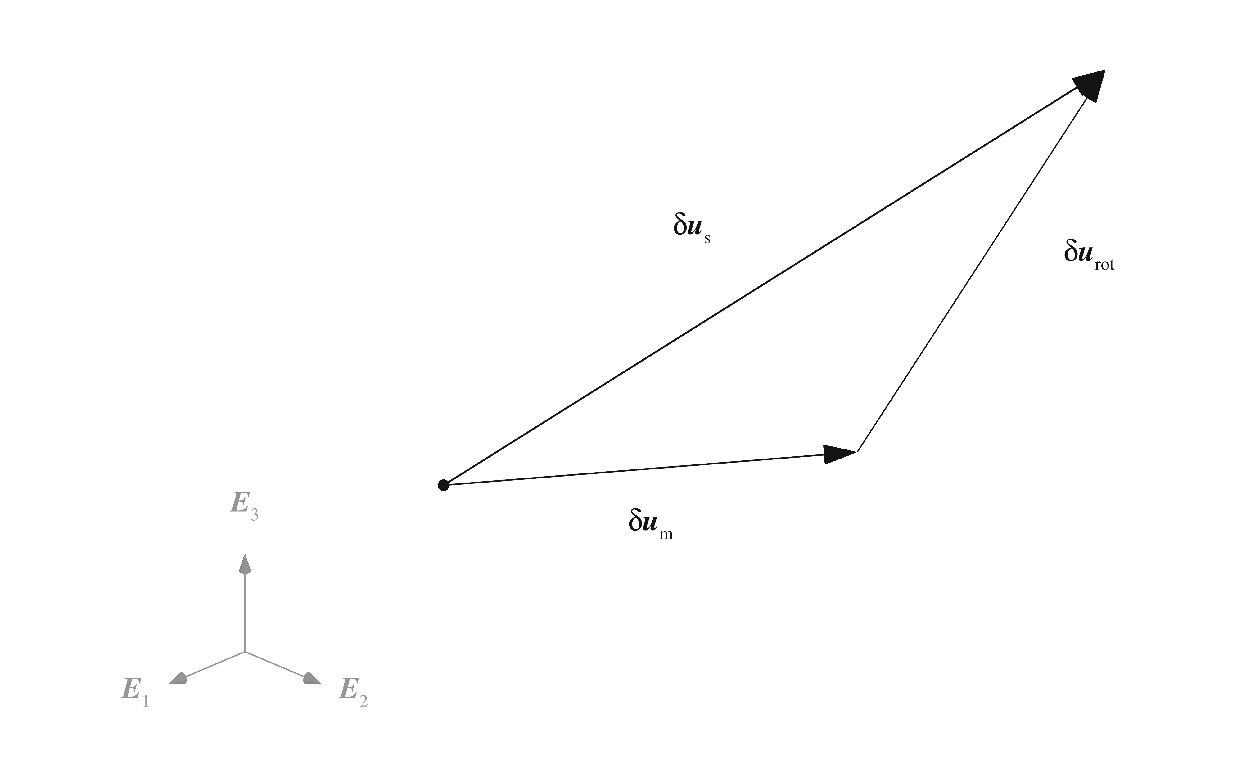
\includegraphics[trim={52.110bp 22.895bp 54.941bp 27.087bp},clip,width=.86\textwidth,height=.31\textheight,keepaspectratio]{figures/tecplot/paper_vinculo_raiz.pdf}
\caption{Compatibilidad incremental entre el maestro $m=H$ y la raíz $s$. Las flechas sucesivas representan $\delta\bm u_m$ y $\delta\bm u_{\rm rot}=\delta\bm\theta_m\times\bm r_s$; la flecha directa representa su suma $\delta\bm u_s$. El punto intermedio incorpora solamente la traslación común del cubo.}\label{fig:vinculo-raiz}
\end{figure*}

Las derivadas se obtienen sustituyendo $\bm r_s$ por $\dot{\bm r}_s=\bm W\bm r_s$ y $\ddot{\bm r}_s=\bm W^2\bm r_s$ en el bloque superior derecho; los restantes bloques derivados son nulos. Al reunir todos los vínculos y condiciones de apoyo se obtiene $\delta\bm q=\bm T(t)\bm z$, donde $\bm z$ contiene únicamente las coordenadas independientes. La matriz $\bm T$ conserva las columnas libres e introduce los bloques $\bm B_s$ en las filas de las raíces. La ecuación~\eqref{eq:fullsystem} se transforma en

\begin{align}
\bm M_r&=\bm T^\tr\bm M\bm T,\nonumber\\
\bm D_r&=\bm T^\tr(\bm D\bm T+2\bm M\dot{\bm T}),\nonumber\\
\bm K_r&=\bm T^\tr(\bm K\bm T+\bm D\dot{\bm T}+\bm M\ddot{\bm T}),\label{eq:dynamicprojection}\\
\bm f_r&=\bm T^\tr\delta\bm f.\nonumber
\end{align}

Una congruencia estática basta solo si $\dot{\bm T}=\ddot{\bm T}=\bm0$. La eliminación cinemática no es un truncamiento modal ni una aproximación de fidelidad.

\subsection{Coordenadas colectivas y cíclicas de las palas}
La transformación de coordenadas de las palas, denominada \emph{multiblade} en la literatura \citep{bir2008}, agrupa los movimientos en una componente colectiva y dos componentes cíclicas. Requiere identificar coordenadas equivalentes en las tres palas, con el mismo orden, posición longitudinal y dirección local. Primero se construye $\bm H(t)$ con bloques $\operatorname{diag}(\bm Q_b,\bm Q_b)$, donde $\bm Q_b=\overline{\bm Q}_{NP_b}$ lleva componentes locales de pala a inerciales. Las raíces ya vinculadas al cubo no se incluyen de nuevo y los bloques de coordenadas que no pertenecen a las palas son identidades.

Para tres valores locales homólogos $\zeta_1,\zeta_2,\zeta_3$, se escribe $[\zeta_1,\zeta_2,\zeta_3]^\tr=\bm B_3[y_0,y_c,y_s]^\tr$, con

\begin{equation}
\bm B_3=\begin{bmatrix}
1&\cos\psi_1&\sin\psi_1\\
1&\cos\psi_2&\sin\psi_2\\
1&\cos\psi_3&\sin\psi_3
\end{bmatrix},\qquad
\psi_b=\psi+\frac{2\pi(b-1)}3.
\end{equation}

La coordenada $y_0$ es el promedio de las tres y $y_c,y_s$ son las amplitudes de los patrones coseno y seno; no representan nuevas deformaciones físicas. Si cada pala posee $n_b$ coordenadas homólogas independientes, se utiliza $\bm B_3\otimes\bm I_{n_b}$, donde $\otimes$ denota aquí el producto de Kronecker entre matrices. Al añadir identidades para el resto de las coordenadas se obtiene $\bm B_{\rm mbc}$. El subíndice $\mathrm{mbc}$ identifica exclusivamente esta transformación. Su combinación con el cambio de base es

\begin{align}
\bm P_{\rm mbc}&=\bm H\bm B_{\rm mbc},\nonumber\\
\dot{\bm P}_{\rm mbc}&=\dot{\bm H}\bm B_{\rm mbc}+\bm H\dot{\bm B}_{\rm mbc},\nonumber\\
\ddot{\bm P}_{\rm mbc}&=\ddot{\bm H}\bm B_{\rm mbc}
+2\dot{\bm H}\dot{\bm B}_{\rm mbc}+\bm H\ddot{\bm B}_{\rm mbc}.
\end{align}

Al introducir $\bm z=\bm P_{\rm mbc}\bm y$, las matrices $\overline{\bm M},\overline{\bm D},\overline{\bm K}$ se obtienen aplicando nuevamente la ecuación~\eqref{eq:dynamicprojection}, con $\bm T$ sustituida por $\bm P_{\rm mbc}$ y matrices de entrada $\bm M_r,\bm D_r,\bm K_r$. El apéndice C presenta la inversa y las derivadas explícitas. Los efectos giroscópicos y las derivadas de este cambio de coordenadas tienen orígenes distintos y se conservan de forma conjunta.

\FloatBarrier
\section{Amortiguamiento y acciones externas}
\subsection{Disipación, gravedad y viento}
El amortiguamiento estructural se representa mediante el modelo de Rayleigh,

\begin{equation}
\bm C_s=\alpha_R\bm M+\beta_R\bm K_{\rm el},\qquad
\zeta_j=\frac{\alpha_R}{2\omega_j}+\frac{\beta_R\omega_j}{2},
\end{equation}

donde $\bm K_{\rm el}$ es la rigidez elástica global de referencia; $\alpha_R$ y $\beta_R$ tienen unidades de $\mathrm{s^{-1}}$ y $\mathrm{s}$. Dos pares de frecuencia angular $\omega_j$ y razón de amortiguamiento $\zeta_j$ determinan ambos coeficientes. Esta relación corresponde a los modos del sistema conservativo de referencia; las razones de amortiguamiento del sistema en operación se obtienen de sus autovalores complejos. A $\bm C_s$ se suman las contribuciones de la conexión, la cimentación y las cargas dependientes de velocidad. La derivada temporal de la masa no representa disipación.

La aceleración gravitatoria es $\bm g=-g\bm E_3$, con $g>0$. Su carga nodal se calcula utilizando la misma distribución de masa. En un elemento de dos nodos,

\begin{equation}
\bm f_{g,e}=\bm M_e^g[\bm g^\tr,\bm0^\tr,\bm g^\tr,\bm0^\tr]^\tr.
\end{equation}

Un cuerpo excéntrico aporta fuerza $m\bm g$ y momento $\bm r_C\times m\bm g$ sobre su punto de referencia. En esta aproximación, la carga gravitatoria se calcula con la geometría nominal y es independiente de la perturbación. Si se actualiza su brazo con la deformación, su derivada respecto de las coordenadas debe incluirse también en la tangente de las acciones externas.

Las acciones aerodinámicas se describen mediante una fuerza distribuida $\bm p_a$ en $\mathrm{N/m}$ y un momento distribuido $\bm m_a$ en $\mathrm{N\,m/m}$. Ambos se refieren al origen seccional y se expresan en la misma base que $\bm N$. La conservación del trabajo virtual determina su carga nodal:

\begin{equation}
\bm f_{a,e}=\int_0^L\bm N^\tr
\begin{bmatrix}\bm p_a\\\bm m_a\end{bmatrix}\dd x.
\end{equation}

La velocidad relativa local es $\bm v_{\rm rel}=\bm v_{\rm aire}-\bm v_{\rm estructura}$, calculada en una base común e incluyendo el movimiento nominal de la pala. La ley aerodinámica relaciona esa velocidad y la orientación seccional con $\bm p_a,\bm m_a$. Si la resultante se aplica en un punto desplazado por $\bm r_a$ respecto del origen de la sección, se incluye el momento $\bm r_a\times\bm p_a$. Los modelos aeroelásticos de \citet{maza2014} proporcionan un antecedente de este acoplamiento; la elección de la ley de flujo es una hipótesis adicional a la formulación estructural. Alrededor del estado de operación,

\begin{align}
\delta\bm f_a&=\bm F_{a,q}\delta\bm q+\bm F_{a,v}\delta\dot{\bm q}
+\delta\bm f_{a,\rm imp},\nonumber\\
\bm K_a&=-\bm F_{a,q},\qquad \bm C_a=-\bm F_{a,v}.
\end{align}

Las matrices $\bm F_{a,q}$ y $\bm F_{a,v}$ son las derivadas de la carga nodal respecto de las coordenadas y sus velocidades; $\delta\bm f_{a,\rm imp}$ reúne las variaciones impuestas del flujo. Una carga es seguidora cuando su dirección cambia con la configuración estructural. Su tangente puede ser no simétrica, por lo que no se supone la existencia de un potencial escalar de posición. La misma ley aerodinámica debe utilizarse para calcular el equilibrio y estas derivadas. Si el flujo tiene memoria, se requieren además sus variables de estado; una dependencia instantánea de posición y velocidad no representa por sí sola esa memoria.

\subsection{Movimiento sísmico de la base}
Sea $\bm\Gamma_f$ la matriz que transmite una traslación uniforme del suelo a todas las coordenadas nodales, incluidas las de apoyo. Para tres componentes de traslación, contiene bloques identidad en las filas traslacionales y ceros en las angulares. La aceleración $\bm a_g(t)=\ddot{\bm u}_g(t)$ produce, en las coordenadas independientes anteriores a la transformación de las palas,

\begin{equation}
\bm f_{s,r}(t)=-\bm P_g(t)\bm a_g(t),\qquad
\bm P_g=\bm T^\tr\bm M\bm\Gamma_f.
\label{eq:seismic}
\end{equation}

Esta forma supone una influencia rígida constante y leyes de fuerza y disipación referidas al movimiento relativo al suelo. Si se parte de una ecuación en coordenadas absolutas, la sustitución $\delta\bm q_{\rm abs}=\bm T\bm z+\bm\Gamma_f\bm u_g$ genera en general la carga

\begin{equation}
-\bm T^\tr(\bm M\bm\Gamma_f\ddot{\bm u}_g
+\bm D\bm\Gamma_f\dot{\bm u}_g+\bm K\bm\Gamma_f\bm u_g).
\end{equation}

Los dos últimos términos solo desaparecen si las matrices correspondientes anulan esa influencia, o si sus leyes se han definido desde el inicio en variables relativas. Una fuerza aerodinámica dependiente de velocidad absoluta exige conservar su contribución correspondiente.

La matriz equivalente $\bm\Gamma_{\rm eff}$, definida por $\bm M_r\bm\Gamma_{\rm eff}=\bm P_g$, reproduce la excitación de base en la ecuación reducida, pero no sustituye a $\bm\Gamma_f$ en la recuperación de movimientos absolutos. La proyección completa retiene los acoplamientos de masa con las coordenadas de apoyo. En coordenadas colectivas y cíclicas se aplica además $\bm P_{\rm mbc}^\tr$ a la carga.

Si la cimentación es flexible, sus coordenadas y matrices deben permanecer en el sistema y la excitación se impone en la interfaz con el suelo. Una rigidez y un amortiguamiento constantes representan una idealización de impedancia; no incorporan por sí solos la no linealidad del suelo ni toda su dependencia frecuencial.

\section{Problemas modal y transitorio}
\subsection{Autovalores y movimientos rígidos}
Para el sistema conservativo detenido, el problema modal es

\begin{equation}
\bm K\bm\phi_j=\omega_j^2\bm M\bm\phi_j,\qquad
\bm\phi_i^\tr\bm M\bm\phi_j=\delta_{ij}.
\end{equation}

El vector $\bm\phi_j$ es el modo de vibración, $\omega_j$ su frecuencia angular y $\delta_{ij}$ el símbolo de Kronecker. La segunda igualdad fija una normalización respecto de la masa. El estado $\bm q_0$ no es un autovector: es la configuración alrededor de la cual se calculan las matrices tangentes. En un sistema conservativo con coeficientes constantes, las vibraciones pueden escribirse como $\delta\bm q(t)=\sum_j\bm\phi_j a_j(t)$, donde $a_j$ son amplitudes modales.
Un elemento libre de doce coordenadas admite las tres traslaciones y tres rotaciones infinitesimales

\begin{equation}
\bm u_i=\bm a+\bm b\times\bm X_i,\qquad \bm\theta_i=\bm b.
\label{eq:rigid}
\end{equation}

En esta expresión, $\bm a$ y $\bm b$ son una traslación y un giro infinitesimal arbitrarios; no son los vectores de posición utilizados en la \hyperref[sec:giro]{deducción de las contribuciones inerciales de la rotación prescrita}. Al elegir sucesivamente sus seis componentes unitarias se forma la matriz de movimientos rígidos $\bm Q_R$. Estos movimientos producen $\bm\varepsilon=\bm0$ y $\bm K_e\bm Q_R=\bm0$. Para las seis rigideces seccionales estrictamente positivas, el complemento deformacional tiene energía positiva y $\operatorname{rank}(\bm K_e)=6$. Si la masa es definida positiva, el elemento libre tiene seis frecuencias analíticamente nulas y seis positivas. Una estructura libre conectada conserva los seis movimientos globales si no presenta mecanismos internos; un empotramiento compatible los elimina.

El núcleo rígido se caracteriza por la ausencia de deformación y de energía elástica. Es distinto del giro nominal impuesto y de las oscilaciones torsionales de una conexión con rigidez positiva.

Para el análisis local en operación, las matrices en coordenadas colectivas y cíclicas se evalúan a un azimut de referencia $\psi_\star$. El caso $\psi_\star=0$ corresponde a la geometría de la figura~\ref{fig:marcos}. La geometría, las matrices y los vínculos se evalúan siempre en el mismo instante. Con $\bm y=\bm\phi e^{\lambda t}$ se obtiene el problema cuadrático de autovalores \citep{tisseur2001},

\begin{equation}
(\lambda^2\overline{\bm M}+\lambda\overline{\bm D}+\overline{\bm K})\bm\phi=\bm0.
\label{eq:QEP}
\end{equation}

Puede resolverse sin invertir explícitamente la masa mediante

\begin{equation}
\begin{bmatrix}\bm0&\I\\-\overline{\bm K}&-\overline{\bm D}\end{bmatrix}
\begin{bmatrix}\bm\phi\\\lambda\bm\phi\end{bmatrix}
=\lambda\begin{bmatrix}\I&\bm0\\\bm0&\overline{\bm M}\end{bmatrix}
\begin{bmatrix}\bm\phi\\\lambda\bm\phi\end{bmatrix}.
\end{equation}

Para un autovalor oscilatorio $\lambda=\sigma+\mathrm i\omega_d$, con $\mathrm i^2=-1$, la frecuencia de oscilación es $f_d=|\omega_d|/(2\pi)$. También pueden definirse $f_n=|\lambda|/(2\pi)$ y $\zeta=-\sigma/|\lambda|$ como parámetros del par complejo. El signo de $\sigma$ indica crecimiento o decaimiento de la perturbación en el sistema local de coeficientes constantes. Si las matrices conservan una dependencia periódica en el tiempo, este problema local no determina por sí solo la estabilidad del movimiento periódico.

\subsection{Proyección de orden reducido}
Una base constante $\bm V$ introduce $\bm y\simeq\bm V\bm\xi$ y produce

\begin{equation}
\bm M_{\rm red}=\bm V^\tr\overline{\bm M}\bm V,\quad
\bm D_{\rm red}=\bm V^\tr\overline{\bm D}\bm V,\quad
\bm K_{\rm red}=\bm V^\tr\overline{\bm K}\bm V.
\end{equation}

La matriz $\bm V$ contiene los vectores de la base elegida y $\bm\xi$ sus amplitudes; la carga se proyecta con $\bm V^\tr$. En el caso conservativo puede elegirse una base modal ortonormal respecto de la masa. Con giro, la selección debe conservar los acoplamientos relevantes para el estado considerado. Una base dependiente del tiempo introduce sus propias derivadas según la ecuación~\eqref{eq:dynamicprojection}. Esta aproximación de menor dimensión se distingue de la eliminación exacta de coordenadas dependientes mediante $\bm T$.

\subsection{Integración y recuperación física}
La integración temporal puede efectuarse en las coordenadas independientes $\bm z$, anteriores a la transformación de las palas. En el análisis local se mantienen constantes $\bm M_r,\bm D_r,\bm K_r$, evaluadas en el mismo estado de operación. Si $t_n$ es el instante de cálculo y $\Delta t=t_{n+1}-t_n$, el método de aceleración media de Newmark se define mediante

\begin{align}
\bm z_{n+1}&=\bm z_n+\Delta t\dot{\bm z}_n
+\tfrac{\Delta t^2}{4}(\ddot{\bm z}_n+\ddot{\bm z}_{n+1}),\nonumber\\
\dot{\bm z}_{n+1}&=\dot{\bm z}_n+\tfrac{\Delta t}{2}
(\ddot{\bm z}_n+\ddot{\bm z}_{n+1}).
\end{align}

La matriz efectiva es $\bm K_r+4\bm M_r/\Delta t^2+2\bm D_r/\Delta t$; se conserva completa, aunque sea no simétrica. El apéndice C presenta el segundo miembro. La estabilidad de un esquema de integración y la estabilidad física del sistema son propiedades diferentes.

Para $\delta\bm q=\bm T(t)\bm z$, la recuperación requiere

\begin{align}
\delta\dot{\bm q}&=\bm T\dot{\bm z}+\dot{\bm T}\bm z,\nonumber\\
\delta\ddot{\bm q}&=\bm T\ddot{\bm z}+2\dot{\bm T}\dot{\bm z}+\ddot{\bm T}\bm z.
\end{align}

Se añade $\bm\Gamma_f\bm a_g$ para recuperar la aceleración absoluta de perturbación; la aceleración centrípeta nominal se incluye por separado si se requiere la aceleración total. Cuando las matrices se evalúan a azimut fijo, también se evalúan $\bm T,\dot{\bm T},\ddot{\bm T}$ en ese azimut: la reconstrucción es local y no representa una trayectoria periódica completa.

Las reacciones se recuperan del residual completo de la ecuación~\eqref{eq:fullsystem}, antes de eliminar apoyos y vínculos. Su proyección sobre coordenadas admisibles es nula. Las resultantes incrementales de seis componentes son
$[\delta\bm n^\tr,\delta\bm m_s^\tr]^\tr=\bm K_s\bm B\bm T_e\delta\bm q_e^g$.
Las resultantes totales incluyen además las del equilibrio $\bm q_0$.

\section{Conclusiones}
La formulación relaciona la descripción material de los componentes con el movimiento nominal, las propiedades seccionales y las ecuaciones discretas de perturbación. El uso de sistemas de referencia definidos y de una convención única de transformación permite distinguir la rotación del rotor de las deformaciones de la torre, la góndola, el cubo y las palas.

La matriz giroscópica se obtiene de la parte antisimétrica del acoplamiento entre velocidades y desplazamientos en la energía cinética. El transporte a ejes fijos y la imposición de vínculos dependientes del tiempo introducen contribuciones adicionales que deben conservarse en conjunto. El equilibrio y la linealización se escriben con los términos inerciales en el primer miembro y las acciones externas en el segundo.

El modelo considera pequeñas deformaciones estructurales, propiedades de masa de referencia y velocidad angular nominal constante. Estas hipótesis permiten formular un análisis local de vibraciones y respuesta transitoria alrededor de un estado de operación. Cuando la excitación o los coeficientes son periódicos, deben conservarse en el problema temporal; una evaluación a azimut fijo no equivale a resolver ese régimen. La formulación establece las relaciones necesarias para incorporar leyes aerodinámicas y de cimentación compatibles con estas hipótesis.

\section{Apéndice A. Matrices e interpolación del elemento}
El orden elemental es $\bm q_e^\ell=[(\bm q_I^\ell)^\tr,(\bm q_J^\ell)^\tr]^\tr$, donde $\bm q_i^\ell=[u_i,v_i,w_i,\theta_{xi},\theta_{yi},\theta_{zi}]^\tr$. La extensión, en índices $(1,7)$, y la torsión, en $(4,10)$, utilizan

\begin{equation}
\bm K_{\rm ax}=\frac{EA}{L}\begin{bmatrix}1&-1\\-1&1\end{bmatrix},\qquad
\bm K_{\rm tor}=\frac{GJ_t}{L}\begin{bmatrix}1&-1\\-1&1\end{bmatrix}.
\end{equation}

Para cada plano se definen

\begin{align}
\phi&=\frac{12EI}{GA_sL^2},&a&=\frac{12EI}{L^3(1+\phi)},\nonumber\\
b&=\frac{6EI}{L^2(1+\phi)},&c&=\frac{(4+\phi)EI}{L(1+\phi)},\nonumber\\
d&=\frac{(2-\phi)EI}{L(1+\phi)}.
\end{align}

El bloque de flexión es

\begin{equation}
\bm K_{\rm fl}=\begin{bmatrix}
a&rb&-a&rb\\rb&c&-rb&d\\-a&-rb&a&-rb\\rb&d&-rb&c
\end{bmatrix}.
\end{equation}

Se emplean $(EI_z,GA_{sy},r=1)$ en índices $(2,6,8,12)$ y $(EI_y,GA_{sz},r=-1)$ en $(3,5,9,11)$. Insertar los cuatro bloques determina todas las entradas de $\bm K_e^\ell$.

Para $s=x/L$ y $\bm p=[1,s,s^2,s^3]$, la interpolación de un plano es $v=\bm p\bm C_v\bm d_y$, $\theta_z=\bm p\bm C_r\bm d_y$, con $\bm d_y=[v_I,\theta_{zI},v_J,\theta_{zJ}]^\tr$ y

\begin{equation}
\bm C_v=\frac1{1+\phi}\begin{bmatrix}
1+\phi&0&0&0\\
-\phi&L(1+\phi/2)&\phi&-L\phi/2\\
-3&-L(2+\phi/2)&3&-L(1-\phi/2)\\
2&L&-2&L
\end{bmatrix},
\end{equation}

\begin{equation}
\bm C_r=\frac1{1+\phi}\begin{bmatrix}
0&1+\phi&0&0\\
-6/L&-(4+\phi)&6/L&-(2-\phi)\\
6/L&3&-6/L&3\\0&0&0&0
\end{bmatrix}.
\end{equation}

Para el otro plano se utilizan $\bm d_z=[w_I,\theta_{yI},w_J,\theta_{yJ}]^\tr$, $\bm S_z=\operatorname{diag}(1,-1,1,-1)$, $w=\bm p\bm C_v\bm S_z\bm d_z$ y $\theta_y=-\bm p\bm C_r\bm S_z\bm d_z$, con el $\phi$ correspondiente. Los campos $u,\theta_x$ se interpolan linealmente. Estas relaciones definen $\bm N$; sus derivadas y los términos de cortante definen $\bm B$.

Para propiedades constantes, cuatro puntos de Gauss integran exactamente los productos de grado máximo seis de masa y giroscopía. La rigidez anterior es cerrada, no obtenida mediante integración reducida. Una formulación de secciones acopladas requiere construir y discretizar su energía general; no se obtiene insertando acoplamientos arbitrarios en estos cuatro bloques.

\section{Apéndice B. Derivadas energéticas}
La relación entre $\dot{\bm\theta}$ y la velocidad angular está dada por~\eqref{eq:jacobiano}. Para verificar la contribución giroscópica, se derivan los términos de velocidad de~\eqref{eq:T2}, con coeficientes constantes:

\begin{align}
\frac{\dd}{\dd t}\frac{\partial\mathcal T_v^{(2)}}{\partial\dot{\bm\eta}}
&=\bm M_6\ddot{\bm\eta}+\bm A_6\dot{\bm\eta},\nonumber\\
\frac{\partial\mathcal T_v^{(2)}}{\partial\bm\eta}
&=\bm A_6^\tr\dot{\bm\eta}.
\end{align}

Al restar se obtiene $\bm M_6\ddot{\bm\eta}+\bm G_{c,6}\dot{\bm\eta}$, con $\bm G_{c,6}=\bm A_6-\bm A_6^\tr$. La parte restante del término inercial se obtiene al aplicar~\eqref{eq:inercia-generalizada} a la energía completa y corresponde a~\eqref{eq:tangente-inercial}. Si los coeficientes dependieran explícitamente del tiempo, aparecerían además $\dot{\bm M}_6\dot{\bm\eta}$ y $\dot{\bm A}_6\bm\eta$.

Para un par externo $\bm\tau$ en componentes nominales, el trabajo virtual es $\delta W=\bm\tau^\tr\bm J_\ell\delta\bm\theta$ y su acción generalizada es $\bm Q_\tau=\bm J_\ell^\tr\bm\tau$. Si $\bm\tau=\bm\tau_0$ permanece constante en esa base, su linealización es $\bm Q_\tau=\bm\tau_0+\tfrac12\Sx{\tau_0}\bm\theta$. Si permanece constante en el cuerpo, $\bm\tau=\bm E\bm\tau_0$ y $\bm Q_\tau=\bm\tau_0-\tfrac12\Sx{\tau_0}\bm\theta$. La matriz que se incorpora al primer miembro es $-\partial\bm Q_\tau/\partial\bm\theta$. Este ejemplo distingue un momento físico de las componentes generalizadas conjugadas al vector de rotación.

La energía corrotacional de la ecuación~\eqref{eq:corot} permite evaluar la fuerza interna y su tangente mediante diferencias centrales. Para incrementos coordenados $h_i$,

\begin{align}
f_i&\simeq\frac{U(\bm q+h_i\bm e_i)-U(\bm q-h_i\bm e_i)}{2h_i},\nonumber\\
K_{ii}&\simeq\frac{U(\bm q+h_i\bm e_i)-2U(\bm q)+U(\bm q-h_i\bm e_i)}{h_i^2},\nonumber\\
K_{ij}&\simeq\frac{U_{++}-U_{+-}-U_{-+}+U_{--}}{4h_ih_j},\quad i\ne j,
\end{align}

donde $U_{\pm\pm}=U(\bm q\pm h_i\bm e_i\pm h_j\bm e_j)$. Los pasos deben respetar la escala y dimensión de las coordenadas. Esta evaluación aproxima las derivadas de una misma energía; no convierte la cinemática aproximada en una viga geométricamente exacta.

Una alternativa lineal de tensión inicial utiliza

\begin{equation}
U_g=\frac{N_0}2\int_0^L[(v')^2+(w')^2]\dd x,
\qquad \bm K_g=N_0\int_0^L\bm N_\perp'{}^\tr\bm N_\perp'\dd x,
\end{equation}

con $N_0>0$ en tracción. Para un plano y la interpolación del Apéndice A,

\begin{equation}
\bm K_g^{(p)}=\frac{N_0}{(1+\phi)^2}\begin{bmatrix}
a_g/L&r/10&-a_g/L&r/10\\
r/10&Lc_g&-r/10&-Ld_g\\
-a_g/L&-r/10&a_g/L&-r/10\\
r/10&-Ld_g&-r/10&Lc_g
\end{bmatrix},
\end{equation}

donde $a_g=\phi^2+2\phi+6/5$, $c_g=\phi^2/12+\phi/6+2/15$ y $d_g=\phi^2/12+\phi/6+1/30$. Esta expresión explica la contribución de la fuerza axial; no se suma a una Hessiana que ya incluye la misma precarga.

\section{Apéndice C. Transformaciones e integración temporal}
La derivada de la masa después de las restricciones es

\begin{align}
\dot{\bm M}_r={}&\dot{\bm T}^\tr\bm M\bm T+\bm T^\tr\dot{\bm M}\bm T
+\bm T^\tr\bm M\dot{\bm T}.
\end{align}

Esta identidad permite separar nuevamente la derivada de masa de la parte antisimétrica de la matriz inercial de velocidad.

La inversa de la transformación colectiva--coseno--seno y las derivadas de la transformación directa son

\begin{equation}
\bm B_3^{-1}=\frac13\begin{bmatrix}
1&1&1\\2\cos\psi_1&2\cos\psi_2&2\cos\psi_3\\
2\sin\psi_1&2\sin\psi_2&2\sin\psi_3
\end{bmatrix},
\end{equation}

\begin{align}
[\dot{\bm B}_3]_{b,:}&=\Omega[0,-\sin\psi_b,\cos\psi_b],\nonumber\\
[\ddot{\bm B}_3]_{b,:}&=-\Omega^2[0,\cos\psi_b,\sin\psi_b].
\end{align}

Para los bloques de pala, $\dot{\bm H}=\bm W_H\bm H$ y $\ddot{\bm H}=\bm W_H^2\bm H$. La matriz $\bm W_H$ repite $\bm W$ en los bloques traslacionales y angulares de las palas, y es nula en las demás coordenadas. Estas derivadas no desaparecen al seleccionar un azimut de evaluación.

Para completar el paso temporal de aceleración media, se define

\begin{align}
\bm K_{\rm eff}&=\bm K_r+\frac4{\Delta t^2}\bm M_r+\frac2{\Delta t}\bm D_r,\nonumber\\
\bm f_{\rm eff}&=\bm f_{n+1}
+\bm M_r\left(\frac4{\Delta t^2}\bm z_n+\frac4{\Delta t}\dot{\bm z}_n+\ddot{\bm z}_n\right)\nonumber\\
&\quad+\bm D_r\left(\frac2{\Delta t}\bm z_n+\dot{\bm z}_n\right),\nonumber\\
\bm K_{\rm eff}\bm z_{n+1}&=\bm f_{\rm eff}.
\end{align}

Aquí $\bm f_{n+1}=\bm f_r(t_{n+1})$ es la carga proyectada en el nuevo instante. Las velocidades y aceleraciones se recuperan de las relaciones de Newmark. El mismo esquema se aplica a un sistema de orden reducido, proyectando también las cargas y las condiciones iniciales \citep{newmark1971}.

\section{Declaración sobre uso de inteligencia artificial}
Se utilizó ChatGPT (OpenAI) como apoyo para organizar y redactar el manuscrito, traducirlo y revisar la correspondencia entre las expresiones matemáticas y el código del proyecto. La herramienta también se utilizó como asistencia en el desarrollo y revisión de la implementación computacional de la formulación. La responsabilidad sobre la exactitud, originalidad e interpretación del contenido corresponde a los autores.

\insertbibliography{Referencias}
\end{document}
